\documentclass{llncs}
%
\usepackage{amsmath}
\usepackage{amssymb}
\usepackage{graphicx}
\usepackage{hyperref}
\usepackage{color,xcolor}
\usepackage{microtype} 
\usepackage{ntheorem}
\usepackage{caption}
\usepackage{subfigure}
\usepackage{array}
\usepackage{graphicx}
\usepackage{multirow}
\usepackage{tikz}
\usepackage{pgfplots}
\pagestyle{plain}
\usetikzlibrary{shapes.geometric, arrows}
% \newtheorem{theorem}{Theorem}
% \newtheorem{lemma}{Lemma}
% \newtheorem*{proof}{\emph{Proof.}}
 \newtheorem{Definition}{Definition}
 \newtheorem{Claim}{Claim}


\begin{document}

\title{An Efficient ECDSA-based Adaptor Signature and Its Two-Party Extension}

\author{Binbin Tu \and Yu Chen \and Min Zhang}

\institute{School of Cyber Science and Technology, Shandong University, Qingdao, China}

\maketitle

\begin{abstract}
%适配器签名是数字签名关于困难关系的扩展,可同时绑定签名授权和秘密泄露两种功能,是解决区块链可扩展性问题的重要技术。
Adaptor signature can tie together transaction authorization and witness extraction and has become an important tool for solving the scalability and interoperability problems in the blockchain. Aumayr et al. first provide the formalization of the adaptor signature and present a provably secure ECDSA-based adaptor signature. However, their scheme requires zero-knowledge proof in the pre-signing phase to ensure the signer works correctly which leads to low efficiency and restricts its functionality extension. 

In this paper, we construct efficient ECDSA-based adaptor signature schemes with offline proof and give security proof based on ECDSA. The pre-signing algorithm of our schemes is similar to the ECDSA signing algorithm except for modifying some parameters. Therefore, our schemes can enjoy the same efficiency and functionality extension as ECDSA. Meanwhile, our schemes can completely reuse the implementation of ECDSA and upgrade existing ECDSA application friendly. Furthermore, we define a two-party adaptor signature with interactive key generation and construct a fast two-party ECDSA-based adaptor signature following the structure of Lindell's two-party ECDSA. Last, we conduct an experimental evaluation, demonstrating that the performance of our ECDSA-based adaptor signature is similar to ECDSA and can compare with the state-of-the-art ECDSA-based adaptor signature.

%额外考虑两方ECDSA-AS的定义,安全性等,参考Lindell‘s TP-ECDSA的定义和安全性,对比最开始的两方ECDSA-AS的设计和NDSS2019上的两方ECDSA-AS的设计,并类似的给出场景应用最后给出代码实现和安全性分析

%后续考虑两方lattice-based AS

\end{abstract}

%区别:之前的证据使用随机数k;本文的证据使用私钥x或者y
%优势如下:1、可以离线执行,很大程度上提升在线预签名的效率;2、这里的zk和消息及随机数无关,所以单独的证明可以签名多个消息,之前的方案不行;3、v1/2的签名结构和ECDSA完全一致,因此,在实现时不需要修改底层的ECDSA的软硬件实现结构,只需要修改签名参数G,Q,对于已采用ECDSA的应用非常友好;4、v2使用y作为证据,因此该证明和x,k无关,在设计分布式构造时很有优势,可直接设计;但是之前的方案和v1在设计分布式时,因为证据是分割的所以需要分布式zk,本身就很困难(解决了A提出的困难问题)

\begin{keywords}
Adaptor signature, Two-party adaptor signature, ECDSA, two-party ECDSA
\end{keywords}

\section{Introduction}

Adaptor signatures (AS), also known as scriptless scripts, are introduced by Poelstra~\cite{Poelstra2017} and recently formalized by Aumayr et al.~\cite{AumayrEEFHMMR20} AS can be seen as an extension over a digital signature with respect to an instance of a hard relation. Namely, the signer can generate a pre-signature with the pre-signing key, message, and an instance of a hard relation, such that the pre-signature can be adapted into a valid full signature by using the witness of the hard relation. The full signature can be verified in the same way as the original verification algorithm. What's more, the witness can be extracted by using the pre-signature and the full signature. Therefore, AS can provide the following properties: (i) only the signer knowing the pre-signing key can generate the pre-signature; (ii)only the user knowing the witness of the hard relation can convert the pre-signature into a valid full signature; (iii) anybody can check the validity of the pre-signature and the corresponding signature and use them to extract the witness of the hard relation. 

Tying together the signature and witness extraction, AS brings about various advantages of reducing the operations on-chain and supporting advanced functionality beyond the limitation of the blockchain’s scripting language. AS has been shown highly useful in many blockchain applications such as payment channels~\cite{AumayrEEFHMMR20,PC2018,DeckerW15,PD2016,AumayrEEFHMMR20a}, payment routing in payment channel networks (PCNs)~\cite{EckeyFHR20,MalavoltaMSKM19,MillerBBKM19,EsginEE20}, atomic swaps~\cite{DeshpandeH20,Gugger20,EsginEE20}, and many others.

Poelstra~\cite{Poelstra2017} first gives a Schnorr-based AS that is limited to cryptocurrencies using Schnorr signatures~\cite{Sch89} and thus is not compatible with those systems, prominently Bitcoin. Then, Moreno-Sanchez and Kate~\cite{Moreno-Sanchez2018} present an ECDSA-based AS and its two-party version, but their schemes are not clear how to prove security. Malavolta et al.~\cite{MalavoltaMSKM19} present protocols for two-party adaptor signatures based on ECDSA~\cite{ECDSA}. However, they do not define AS as a stand-alone primitive and formalize the security definition for the threshold primitive and hence security for their schemes has not been analyzed completely. Until Aumayr et al.~\cite{AumayrEEFHMMR20} first formalize AS as a standalone primitive and prove the security of their ECDSA-based AS based on the strong unforgeability of positive ECDSA in the Universal Composability (UC) framework~\cite{Canetti01}. They exquisitely modify the hard relation in~\cite{Moreno-Sanchez2018}, by adding zero-knowledge proof such that they can extract the witness in the random model~\cite{Fischlin05}, namely ``self-proving structure''. However, their ECDSA-based AS requires another zero-knowledge proof in the pre-signing phase to ensure that the signer works correctly, which leads to low efficiency and restricts the functionality extension compared with original ECDSA~\cite{ECDSA}, such as two-party~\cite{Lin17,CCLST19,YuenCX21} or threshold extension~\cite{GGN16,BGG17,LN18,GG18,DKLs19}. Then, Erwig et al.~\cite{ErwigFHM021} define two-party adaptor signature schemes with aggregatable public keys and give a generic transformation from identification schemes. However, their definition is unsuitable for two-party ECDSA-based AS.  

%根据上述分析:
%1:缺少适用于两方ECDSA适配器签名的交互式密钥生成的两方适配器签名的定义
%2:现有ECDSA方案结构不易于进行两方扩展,且预签名效率较低

Unfortunately, the constructions of ECDSA-based AS and the formalization of two-party AS given in existing works have two limitations: (i) the state-of-the-art ECDSA-based AS~\cite{AumayrEEFHMMR20} is not entirely satisfactory, such as it is not easy to be extended into two-party, and zero-knowledge proof in the pre-signature phase leads to low efficiency; (ii) missing the formalization of two-party adapter signature with an interactive key generation that is suitable for two-party ECDSA-based AS. Motivated by above discussions, we ask the following challenging question:\\

\begin{minipage}{0.9\textwidth}
\centering
\emph{Is it possible to define a two-party adaptor signature with interactive key generation and construct an efficient ECDSA-based adaptor signature scheme that is easy to be extended into two-party?}
\end{minipage}


\subsection{Our Contributions}

In this paper, we affirmatively answer the previous questions. First, we propose an ECDSA-based AS (ECDSA-AS) and use ``self-proving structure''~\cite{AumayrEEFHMMR20} $I_Y=(Y, \pi_Y)$ to prove the security based on positive ECDSA in UC framework~\cite{Canetti01}. And then, we observe that the zero-knowledge proof used in the pre-signing phase is independent of the message and random number, so we can consider the ``offline-proof technique'' to improve the efficiency of the online pre-signing phase, and construct two efficient ECDSA-AS schemes. For convenience, we denote our two efficient ECDSA-AS schemes by ECDSA-ASv1 and ECDSA-ASv2. The difference between the two schemes is to use different witnesses to prove similar hard relations. ECDSA-ASv1 uses the pre-signing key $x$ as a witness to prove the hard relation $((G, Q=xG, Y, Z=xY), x)$ satisfies equality of discrete logarithms. ECDSA-ASv2 uses the witness $y$ of hard relation $(I_Y,y)$ as a witness to prove the hard relation $((G, Y=yG, Q, Z=yQ), y)$ satisfies equality of discrete logarithms. With the offline zero-knowledge proof, the online pre-signing algorithm of our ECDSA-ASv1/2 is similar to the original ECDSA signing algorithm except for modifying some parameters by using $(Z, Y)$ as verification key and base point instead of $(Q, G)$ used in ECDSA. Therefore, our schemes can enjoy the same efficiency and functionality extension as ECDSA. Furthermore, we define two-party AS with interactive key generation and construct a fast two-party ECDSA-AS based on ECDSA-ASv2 following the structure of Lindell's two-party ECDSA~\cite{Lin17}.

\begin{trivlist}
\item \textbf{Self-proving structure.} Intuitively speaking, for hard relation $(Y=yG,y)$ embedded in AS, our schemes also use ``self-proving structure'' following~\cite{AumayrEEFHMMR20} to ensure provable security. That is, we add an additional proof $\pi_Y\leftarrow \mathsf{P}(Y,y)$ in the hard relation $(I_Y=(Y, \pi_Y),y)$, where $\mathsf{V}(Y,\pi_Y)\rightarrow 1$, $\mathsf{P}$ and $\mathsf{V}$ denote the proving and verification algorithm in the proof systems. Benefiting from the above modification, upon receiving an instance $I_Y= (Y,\pi_Y)$, there is an extractor that can extract the witness $y$ from $\pi_Y$ in the random oracle model~\cite{AumayrEEFHMMR20}, online extractor as introduced in~\cite{Fischlin05}. Thus, in the security proof, the simulator can extract the witness $y$ and take advantage of the ECDSA signing oracle to simulate the pre-signing oracle. 
\end{trivlist}

\begin{trivlist}
\item \textbf{Offline proof.} In the pre-signing algorithm, our ECDSA-AS proves the hard relation $((G, Q, Y, Z),x)$ satisfies equality of discrete logarithms, that is, there exists the witness $x$ that is pre-signing key, such that $Q=xG$ and $Z=xY$. However, in~\cite{AumayrEEFHMMR20}, they prove the hard relation $((G, K, Y, \hat{K}),k)$ satisfies equality of discrete logarithms, that is, there exists the witness $k$ that is a random number used in the pre-signing algorithm, such that $K=kG$ and $\hat{K}=kY$. According to the structure $Z=xY=yQ$, our ECDSA-AS can also prove the hard relation $((G, Y, Q, Z), y)$ satisfies equality of discrete logarithms, that is, there exists the witness $y$ that is the witness of hard relation $(I_Y=(Y, \pi_Y),y)$, such that $Y=yG$ and $Z=yQ$.

Compared with~\cite{AumayrEEFHMMR20}, our zero-knowledge proofs are independent of the message $m$ and the random number $k$ used in the pre-signature, so the proofs can be executed offline. At the same time, for same hard relation $(I_Y=(Y, \pi_Y),y)$, one zero-knowledge proof for $((G, Q, Y, Z), x)$ or $((G, Y, Q, Z),y)$ can be used to pre-signing many messages, but due to using the random number $k$ as the witness in~\cite{AumayrEEFHMMR20}, the size of zero-knowledge proof is linearly related to the number of pre-signatures.
\end{trivlist}
\begin{trivlist}
\item \textbf{Two-party extension.} ECDSA-AS~\cite{AumayrEEFHMMR20} uses the random number $k$ as the witness that should be shared to many parties in constructing two-party or threshold ECDSA-AS, so the zero-knowledge proof of proving the equality of discrete logarithms for $((G, K, Y, \hat{K}),k)$ should be distributed, which may be difficult to achieve. 

Because the pre-signing algorithm of our scheme is similar to the original ECDSA signing algorithm, the signer can run ECDSA signing algorithm by using $Y$ as a base point and $Z$ as a verification key instead of $G$ and $Q$ to generate the pre-signature. Our schemes can enjoy the same functionality extension as ECDSA. In particular, in ECDSA-ASv2, the two zero-knowledge proofs of hard relations $(I_Y,y)$ and $((G, Y, Q, Z),y)$ are generated by the hard relation chooser, hence the signer only runs the ECDSA signing algorithm with modified parameter $(Y, Z)$ to generate the pre-signature. Therefore, ECDSA-ASv2 can easily be transformed into two-party~\cite{Lin17,CCLST19,YuenCX21} or even threshold version~\cite{GGN16,BGG17,LN18,GG18,DKLs19} following existing ECDSA extension. 

Since most efficient two-party ECDSA requires interactive key generation, the definition of two-party AS with aggregatable public keys~\cite{ErwigFHM021} is unsuitable for two-party ECDSA-AS. Therefore, we define two-party AS with interactive key generation following the definition of two-party signature~\cite{Lin17,CCLST19} and two-party AS~\cite{ErwigFHM021}, and then transform our ECDSA-ASv2 into a provably secure two-party ECDSA-AS. 
\end{trivlist}

\begin{trivlist}
\item \textbf{Performance.} Benefiting from holding the original ECDSA signing structure, our schemes can enjoy the same efficiency and completely reuse the hardware and software implementation of ECDSA except for modifying parameters, so it is friendly to upgrade existing ECDSA application. Then, We recall ECDSA-AS~\cite{Moreno-Sanchez2018,AumayrEEFHMMR20}, and show the theoretical analysis of our ECDSA-AS. Our schemes can achieve the same level of efficiency as ECDSA and are more efficient than the state-of-the-art ECDSA-AS~\cite{Moreno-Sanchez2018,AumayrEEFHMMR20}, in particular, ECDSA-ASv1/2 only computes once point multiplication operation, while ECDSA-AS in~\cite{Moreno-Sanchez2018,AumayrEEFHMMR20} need four times point multiplication operation in online pre-signing phase. Last, we realize our schemes based on the OpenSSL, and the running times of all algorithms are the level of microseconds. The experimental results show that our proposed schemes are practical.
\end{trivlist}

\section{Preliminaries}
\subsection{Notations}

For $n\in \mathbb{N}$, $1^\lambda$ denotes the string of $\lambda$ ones. Throughout, we use $\lambda$ to denote the security parameter. A function is negligible in $\lambda$, written $\mathsf{negl}(\lambda)$, if it vanishes faster than the inverse of any polynomial in $\lambda$. We denote a probabilistic polynomial-time algorithm by PPT. If $S$ is a set then $s\leftarrow S$ denotes the operation of sampling an element $s$ of $S$ at random.

\subsection{Adaptor Signature Scheme}~\label{Adaptor Signature Scheme}

An adaptor signature scheme~\cite{AumayrEEFHMMR20} w.r.t. a hard relation $\mathsf{R}=\{Y,y\}$ and a signature scheme $\sum = (\mathsf{Gen}, \mathsf{Sign}, \mathsf{Vrfy})$ consists of four algorithms $\Pi_{\mathsf{R},\sum} = ($$\mathsf{pSign}$, $\mathsf{pVrfy}$, $\mathsf{Adapt}$, $\mathsf{Ext})$ defined as:


\begin{itemize}
\item $\mathsf{pSign}_{sk}(m,Y)\rightarrow \hat{\sigma}$: on input a pre-signing key $sk$, an instance $Y$ and a message $m \in \{0, 1\}^*$, outputs a pre-signature $\hat{\sigma}$.

\item $\mathsf{pVrfy}_{vk}(m,Y,\hat{\sigma})\rightarrow 0/1$: on input a verification key $vk$, a pre-signature $\hat{\sigma}$, an instance $Y$ and a message $m \in \{0, 1\}^*$, outputs a bit $b\in \{0, 1\}$.

\item $\mathsf{Adapt}(\hat{\sigma},y)\rightarrow \sigma$: on input a pre-signature $\hat{\sigma}$ and a witness $y$, outputs a signature $\sigma$.

\item $\mathsf{Ext}(\sigma,\hat{\sigma},Y)\rightarrow y$: on input a signature $\sigma$, a pre-signature $\hat{\sigma}$ and an instance $Y$, outputs a witness $y$ such that $(Y,y)\in \mathsf{R}$, or $\bot$.
\end{itemize}

In addition to the standard signature correctness, an AS has to satisfy pre-signature correctness. Informally, it guarantees that an honestly generated pre-signature w.r.t. an instance $Y \in \mathsf{R}$ is a valid pre-signature and can be completed into a valid signature from which a witness for $Y$ can be extracted.

\begin{Definition}\emph{(Pre-signature correctness)}. An adaptor signature scheme $\Pi_{\mathsf{R},\sum}$ satisfies pre-signature correctness if for every $\lambda$, every message $m \in \{0,1\}^*$ and every statement/witness pair $(Y, y) \in \mathsf{R}$, the following holds:
\end{Definition}

\begin{equation*}
\begin{aligned}
\Pr\left[
\begin{array}{c|c}
\mathsf{pVrfy}_{vk}(m,Y,\hat{\sigma})\rightarrow 1 & \mathsf{Gen}(1^\lambda)\rightarrow (sk,vk) \\
\wedge & \mathsf{pSign}_{vk}(m,Y)\rightarrow \hat{\sigma}\\               
\mathsf{Vrfy}_{vk}(m,\sigma)\rightarrow 1  & \mathsf{Adapt}(\hat{\sigma},y)\rightarrow \sigma\\
\wedge  & \mathsf{Ext}(\sigma,\hat{\sigma},Y)\rightarrow y'\\
(Y,y')\in \mathsf{R} & \\
\end{array}
\right]=1
\end{aligned}
\end{equation*}

We now define the security properties of an AS scheme. We begin with the notion of unforgeability which is similar to the definition of existential unforgeability under chosen message attacks but additionally requires that producing a forgery $\sigma$ for some message $m$ is hard even given a pre-signature on $m$ w.r.t. an instance $Y \in \mathsf{R}$. Let us emphasize that allowing the adversary to learn a pre-signature on the forgery message $m$ is crucial since for our applications unforgeability needs to hold even in case the adversary learns a pre-signature for $m$ without knowing a corresponding witness for $Y$. We formally define the existential unforgeability under chosen message attack for AS (aEUF–CMA).

\begin{Definition}\emph{(aEUF–CMA security).}~\label{aEUF-CMA security definition}
An adaptor signature scheme $\Pi_{\mathsf{R},\sum}$ is aEUF–CMA secure if for every PPT adversary $\mathcal{A}$ there exists a negligible function $\mathsf{negl}$ such that: $\Pr[\text{aSigForge}_{\mathcal{A},\Pi_{\mathsf{R},\sum}}(\lambda) = 1] \leq \mathsf{negl}(\lambda)$, where the experiment $\text{aSigForge}_{\mathcal{A},\Pi_{\mathsf{R},\sum}}$ is defined as follows:
\end{Definition}

\begin{center}
\fbox{
\begin{tabular}{lll}
 $\text{aSigForge}_{\mathcal{A},\Pi_{\mathsf{R},\sum}}(\lambda)$ & \ \  & $\mathcal{O}_{\text{Sign}_{sk}}(m)$ \\
\cline{1-1} \cline{3-3}

 $\mathcal{Q}=\emptyset$ & \ \  & $\sigma\leftarrow \mathsf{Sign}_{sk}(m)$ \\

 $(vk,sk)\leftarrow \mathsf{Gen}(1^\lambda)$ & \ \  & $\mathcal{Q}=\mathcal{Q}\cup \{m\}$ \\

 $m\leftarrow \mathcal{A}^{\mathcal{O}_{\text{Sign}_{sk}}(\cdot),\mathcal{O}_{\text{pSign}_{sk}}(\cdot)}(vk)$ & \ \  & return $\sigma$ \\
 $(Y,y)\leftarrow \mathsf{GenR}(1^\lambda)$ & \ \  &  \\
  $\hat{\sigma}\leftarrow \mathsf{pSign}_{sk}(m,Y)$ & \ \  & $\mathcal{O}_{\text{pSign}_{sk}}(m,Y)$ \\
 \cline{3-3}

 $\sigma\leftarrow \mathcal{A}^{\mathcal{O}_{\text{Sign}_{sk}}(\cdot),\mathcal{O}_{\text{pSign}_{sk}}(\cdot)}(\hat{\sigma},Y)$ & \ \  & $\hat{\sigma}\leftarrow \mathsf{pSign}_{sk}(m,Y)$ \\

 return $(m\notin \mathcal{Q} \wedge \mathsf{Vrfy}_{vk}(m,\sigma))$ & \ \  & $\mathcal{Q}=\mathcal{Q}\cup \{m\}$  \\

  & \ \  & return $\hat{\sigma}$  \\
\end{tabular}}
\end{center}

As discussed above, AS guarantees that a valid pre-signature w.r.t. $Y$ can be completed to a valid signature if and only if the corresponding witness $y$ for $Y$ is known. An additional property that we will require is that any valid pre-signature w.r.t. $Y$ (possibly produced by a malicious signer) can be completed into a valid signature using the witness y with $(Y, y) \in \mathsf{R}$. Notice that this property is stronger than the pre-signature correctness property, since we require that even maliciously produced pre-signatures can always be completed into valid signatures. The next definition formalizes the above discussion.

\begin{Definition}\emph{(Pre-signature adaptability).} An adaptor signature scheme $\Pi_{\mathsf{R},\sum}$ satisfies pre-signature adaptability if for any $\lambda$, any message $m \in \{0, 1\}^*$ , any statement/witness pair $(Y,y) \in \mathsf{R}$, any key pair $(vk,sk) \leftarrow \mathsf{Gen}(1^\lambda)$ and any pre-signature $\hat{\sigma}$ with $\mathsf{pVrfy}_{vk}(m,Y,\hat{\sigma})\rightarrow 1$, we have  $\Pr[\mathsf{Vrfy}_{vk}(m$, $\mathsf{Adapt}(\hat{\sigma}$, $y))\rightarrow 1] = 1$.
\end{Definition}

The aEUF–CMA security together with the pre-signature adaptability ensures that a pre-signature for $Y$ can be transferred into a valid signature if and only if the corresponding witness $y$ is known. The last property that we are interested in is witness extractability. Informally, it guarantees that a valid signature/pre-signature pair $(\sigma, \hat{\sigma})$ for message/statement $(m, Y)$ can be used to extract the corresponding witness $y$.


\begin{Definition}\emph{(Witness extractability).} An adaptor signature scheme $\Pi_{\mathsf{R},\sum}$ is witness extractable if for every PPT adversary $\mathcal{A}$, there exists a negligible function $\mathsf{negl}$ such that the following holds: 

$$\Pr[\text{aWitExt}_{\mathcal{A},\Pi_{\mathsf{R},\sum}}(\lambda) = 1] \leq \mathsf{negl}(\lambda),$$
where the experiment $\text{aWitExt}_{\mathcal{A},\Pi_{\mathsf{R},\sum}}$ is defined as follows
\end{Definition}

Let us stress that while the witness extractability experiment aWitExt looks fairly similar to the experiment aSigForge, there is one crucial difference; namely, the adversary is allowed to choose the forgery instance $Y$. Hence, we can assume that he knows a witness for $Y$ so he can generate a valid signature on the forgery message $m$. However, this is not sufficient to win the experiment. The adversary wins only if the valid signature does not reveal a witness for $Y$.

\begin{center}
\fbox{
\begin{tabular}{lll}
 $\text{aWitExt}_{\mathcal{A},\Pi_{\mathsf{R},\sum}}(\lambda)$ & \ \  & $\mathcal{O}_{\text{Sign}_{sk}}(m)$ \\
\cline{1-1} \cline{3-3}

 $\mathcal{Q}=\emptyset$ & \ \  & $\sigma\leftarrow \mathsf{Sign}_{sk}(m)$ \\

 $(vk,sk)\leftarrow \mathsf{Gen}(1^\lambda)$ & \ \  & $\mathcal{Q}=\mathcal{Q}\cup \{m\}$ \\

 $(m,Y)\leftarrow \mathcal{A}^{\mathcal{O}_{\text{Sign}_{sk}}(\cdot),\mathcal{O}_{\text{pSign}_{sk}}(\cdot)}(vk)$ & \ \  & return $\sigma$ \\
 $\hat{\sigma}\leftarrow \mathsf{pSign}_{sk}(m,Y)$ & \ \  &  \\
 $\sigma \leftarrow \mathcal{A}^{\mathcal{O}_{\text{Sign}_{sk}}(\cdot),\mathcal{O}_{\text{pSign}_{sk}}(\cdot)}(\hat{\sigma})$  & \ \  & $\mathcal{O}_{\text{pSign}_{sk}}(m,Y)$ \\
 \cline{3-3}

 $y'\leftarrow \mathsf{Ext}(\sigma,\hat{\sigma},Y)$ & \ \  & $\hat{\sigma}\leftarrow \mathsf{pSign}_{sk}(m,Y)$ \\

 return $(m\notin \mathcal{Q} \wedge (Y,y')\notin \mathsf{R}$ & \ \  & $\mathcal{Q}=\mathcal{Q}\cup \{m\}$  \\

 $\wedge \mathsf{Vrfy}_{vk}(m,\sigma))$ & \ \  & return $\hat{\sigma}$  \\

\end{tabular}}
\end{center}


\subsection{ECDSA} 
We review the ECDSA scheme~\cite{ECDSA} $\sum=(\mathsf{Gen}, \mathsf{Sign}, \mathsf{Vrfy})$ on a message $m\in \{0,1\}^*$ as follows.  Let $\mathbb{G}$ be an Elliptic curve group of order $q$ with base point (generator) $G$ and let $pp=(\mathbb{G},G,q)$ be the public parameter. 
\begin{itemize}
\item $\mathsf{Gen}(pp)\rightarrow (Q,x)$: The key generation algorithm uniformly chooses a secret signing key $x\leftarrow \mathbb{Z}_q$, and calculates the verification key $Q=x\cdot G$, and outputs $(sk=x,vk=Q)$.
\item $\mathsf{Sign}_{sk}(m)\rightarrow (r,s)$. The signing algorithm chooses $k\leftarrow \mathbb{Z}_q$ randomly and computes $r = f(kG)$ and $s = k^{-1}(h(m) + rx)$, where $h: \{0,1\}^* \rightarrow \mathbb{Z}_q$ is a hash function modeled as a random oracle and $f: \mathbb{G} \rightarrow \mathbb{Z}_q$ is defined as the projection to the $x$-coordinate.
\item $\mathsf{Vrfy}_{vk}(m,\sigma)\rightarrow 0/1$. The verification algorithm computes $r'=f(s^{-1}\cdot (m'\cdot G+r\cdot Q))$. If $r=r'\bmod q$, outputs $1$, otherwise, outputs $0$.
\end{itemize}

According to the structure of ECDSA, if $(r, s)$ is a valid signature for $m$, then so is $(r,-s)$. Therefore, $\sum$ does not satisfy SUF-CMA security which we need to prove the security of ECDSA-AS. In order to tackle this problem, we recall the Positive ECDSA scheme which guarantees that if $(r, s)$ is a valid signature, then $|s| \leq (q - 1)/2$. The positive ECDSA has already been used in other works such as~\cite{Lin17}.

\section{ECDSA-based Adaptor Signature}~\label{ECDSA-based Adaptor Signature}

In this section, we present a construction of ECDSA-AS $\Pi_{\mathsf{R},\sum}$ $= ($$\mathsf{pSign}$, $\mathsf{pVrfy}$, $\mathsf{Adapt}$, $\mathsf{Ext})$ w.r.t. a hard relation $\mathsf{R}$ and a ECDSA signature $\sum = (\mathsf{Gen}$, $\mathsf{Sign}$, $\mathsf{Vrfy})$. Formally, we define hard relations $\mathsf{R}= \{(I_Y=(Y,\pi_Y), y) | Y = yG \wedge \mathsf{V}(I_Y) = 1\}$ and $\mathsf{R}_Z=\{(I_Z=(G,Q,Y,Z), x) | Q = xG \wedge Z=xY\}$, and denote by $\mathsf{P}$ the prover and by $\mathsf{V}$ the verifier of the proof system.

\begin{itemize}
\item $\mathsf{pSign}_{(vk,sk)}(m,I_Y)\rightarrow \hat{\sigma}$: on input a key-pair $(vk,sk)=(Q,x)$, a message $m$ and an instance $I_{Y}=(Y,\pi_Y)$, the algorithm computes $Z=xY$, runs $\pi_Z\leftarrow \mathsf{P}(I_Z=(G,Q,Y,Z),x)$, and chooses $k\leftarrow \mathbb{Z}_q$, computes $r=f(kY)$, $\hat{s}=k^{-1}(h(m)+rx) \bmod q$ and outputs $\hat{\sigma}=(r,\hat{s},Z,\pi_Z)$.

\item $\mathsf{pVrfy}_{vk}(m,I_Y,\hat{\sigma})\rightarrow 0/1$: on input the verification key $vk=Q$, a message $m$, an instance $I_{Y}$, and a pre-signature value $\hat{\sigma}$, the algorithm outputs $\bot$ if $\mathsf{V}(I_{Z})\rightarrow 0$, otherwise, it computes $r'=f(\hat{s}^{-1}\cdot (h(m)\cdot Y+r\cdot Z))$, and if $r'=r$, outputs $1$, else outputs $0$.

\item $\mathsf{Adapt}(y,\hat{\sigma})\rightarrow \sigma$: on input the witness $y$, and pre-signature $\hat{\sigma}$, the algorithm computes $s=\hat{s}\cdot y^{-1} \bmod q$ and outputs the signature $\sigma=(r,s)$.

\item $\mathsf{Ext}(\sigma,\hat{\sigma},I_Y)\rightarrow y$: on input the signature $\sigma$, the pre-signature $\hat{\sigma}$ and the instance $I_{Y}$, the algorithm computes $y=\hat{s}/s \bmod q$. If $(I_Y, y)\in \mathsf{R}$, it outputs $y$, else outputs $\bot$.
\end{itemize}

\begin{figure*}[!htbp]
\begin{center}
\fbox{
\begin{tabular}{lll}
$\mathsf{pSign}_{(vk,sk)}(m,I_Y)$&\ \ & $\mathsf{pVrfy}_{vk}(m,I_Y,\hat{\sigma})$  \\
\cline{1-1} \cline{3-3}

$(vk,sk)=(Q,x),Z=xY$&\ \  & if $\mathsf{V}(I_Z)\rightarrow 0$    \\

$\mathsf{P}(I_Z,x)\rightarrow \pi_Z$&\ \  & outputs $\bot$.\\

$k\leftarrow \mathbb{Z}_q$&\ \   &  else, $r'=f(\hat{s}^{-1}\cdot h(m)\cdot Y+\hat{s}^{-1}\cdot r\cdot Z))$  \\

$r=f(kY)$&\ \   &  If $r'=r$, output $1$  \\

$\hat{s}=k^{-1}(h(m)+rx) \bmod q$&\ \  &  else, output $0$. \\

return $\hat{\sigma}=(r,\hat{s},Z,\pi_Z)$&\ \   & return $0/1$  \\
&\ \ &\\

$\mathsf{Adapt}(y,\hat{\sigma})$&\ \  &$\mathsf{Ext}(\sigma,\hat{\sigma},I_Y)\rightarrow y$ \\
\cline{1-1} \cline{3-3}

$\hat{\sigma}=(r,\hat{s},Z,\pi_Z)$&\ \  &$\sigma=(r,s),\hat{\sigma}=(r,\hat{s},Z,\pi_Z)$ \\

$s=\hat{s}\cdot y^{-1} \bmod q$&\ \  &$y=\hat{s}/s \bmod q$\\

return $\sigma=(r,s)$&\ \  &If $(I_Y, y)\in \mathsf{R}$, it returns $y$,\\

&\ \  &else, it returns $\bot$\\


\end{tabular}}
\caption{ECDSA-based adaptor signature scheme}
\label{ECDSA-based adaptor signature scheme}
\end{center}
\end{figure*}

% Note that it is possible to check the validity of the proof in an offline phase. When $m$ is received, the signer can use $Y$ to run ECDSA signing algorithm to generate the pre-signature instead of $G$. As we can see, if we run $\mathsf{V}(I_{Y})$ offline, the $\mathsf{pSign}$ algorithm and $\mathsf{pVrfy}$ algorithm are similar to the original ECDSA signing and verification algorithm except that using $Y$ and $Z$ instead of $G$ and $Q$.

Note that in the pre-signing phase, our ECDSA-AS uses the pre-signing key $x$ as the witness to prove the hard relation $((G, Q=xG, Y=yG, Z=xY), x)$ satisfies equality of discrete logarithms, while in~\cite{AumayrEEFHMMR20}, they use the random number $k$ as the witness to prove the hard relation $((G, K=kG, Y=yG, \hat{K}=kY), k)$ satisfies equality of discrete logarithms. With this change, the zero-knowledge proof in our scheme can be executed offline, and in the online phase, the pre-signing algorithm is similar to the original ECDSA signing algorithm except for using $(Z, Y)$ as verification key and base point instead of $(Q, G)$. In addition, for the same hard relation $(I_Y,y)$, our scheme only needs one zero-knowledge proof for pre-signing many different messages, but in~\cite{AumayrEEFHMMR20}, the zero-knowledge proof is linearly related to the number of pre-signatures.

\begin{theorem}
Assuming that the positive ECDSA signature $\sum$ is SUF-CMA secure and $\mathsf{R}$ is a hard relation, the ECDSA-based adaptor signature $\Pi_{\mathsf{R},\sum}$ as defined in fig.~\ref{ECDSA-based adaptor signature scheme} is secure in random oracle model.
\end{theorem}

We prove that our ECDSA-AS scheme in fig.~\ref{ECDSA-based adaptor signature scheme} satisfies pre-signature adaptability, pre-signature correctness, aEUF–CMA security, and witness extractability as follows. 

\begin{lemma}\emph{(Pre-signature adaptability)}\label{Pre-signature adaptability} 
The ECDSA-based adaptor signature scheme $\Pi_{\mathsf{R},\sum}$ satisfies pre-signature adaptability.
\end{lemma}

\begin{proof}
For any $(I_Y,y)\in \mathsf{R}$, $m\in \{0,1\}^*$, $G,Q,Y,Z\in \mathbb{G}$ and $\hat{\sigma} = (r,\hat{s},Z,\pi_Z)$. For $\mathsf{pVrfy}_{vk}(m,I_Y,\hat{\sigma})\rightarrow 1$. That is, $Y=yG,Z=xY=yQ=xyG$, $\hat{K}=(h(m)\cdot\hat{s}^{-1})Y+r\cdot\hat{s}^{-1}Z=kY$, $r'=f(\hat{K})=f(kY)=r$. 

By definition of $\mathsf{Adapt}$, we know that $\mathsf{Adapt}(\hat{\sigma}, y)\rightarrow \sigma$, where $\sigma=(r,s), s = \hat{s}\cdot y^{-1} = (yk)^{-1}(h(m)+rx)\bmod q$. Hence, we have 
$$K'=(h(m)\cdot s^{-1})G+r\cdot s^{-1}Q=kY.$$ 
Therefore, $r'=f(K')=f(kY)=r$. That is $\mathsf{Vrfy}_{vk}(m,\sigma)\rightarrow 1$.
\end{proof}

\begin{lemma}\emph{(Pre-signature correctness)}~\label{Pre-signature correctness} The ECDSA-based adaptor signature scheme $\Pi_{\mathsf{R},\sum}$ satisfies pre-signature correctness.
\end{lemma}

\begin{proof}
For any $x,y\in \mathbb{Z}_q$, $Q=xG,Y=yG$ and $m\in \{0,1\}^*$.  
For $\mathsf{pSign}_{(vk,sk)}(m$, $I_Y)\rightarrow$ $\hat{\sigma}$ $=(r$, $\hat{s}$, $Z$, $\pi_Z)$, it holds that $Y=yG, Z=xY$, $\hat{s}=k^{-1}(h(m)+rx) \bmod q$ for some $k\leftarrow \mathbb{Z}_q$. Set $\hat{K}=(h(m)\cdot\hat{s}^{-1})Y+r\cdot\hat{s}^{-1}Z=kY.$

Therefore, $r'=f(\hat{K})=f(kY)=r$, we have $\mathsf{pVrfy}_{vk}(m,I_Y,\hat{\sigma})\rightarrow 1$. By Lemma $1$, this implies that $\mathsf{Vrfy}_{vk}(m,\sigma)\rightarrow 1$, for $\mathsf{Adapt}(\hat{\sigma}, y)\rightarrow \sigma=(r,s)$. By the definition of $\mathsf{Adapt}$, we know that $s=\hat{s}\cdot y^{-1}$ and hence
$$\mathsf{Ext}(\sigma,\hat{\sigma},I_Y)=\hat{s}/s=\hat{s}/(\hat{s}/y)=y.$$
\end{proof}

\begin{lemma}\emph{(aEUF–CMA security)}~\label{aEUF-CMA security} Assuming that the positive ECDSA signature scheme $\sum$ is SUF–CMA secure and $\mathsf{R}$ is a hard relation, the ECDSA-based adaptor signature scheme $\Pi_{\mathsf{R},\sum}$ as defined above is aEUF–CMA secure.
\end{lemma}

\begin{proof}
We prove the aEUF–CMA security of the ECDSA-AS by reduction to strong unforgeability of positive ECDSA signatures. Our proof works by showing that, for any PPT adversary $\mathcal{A}$ breaking aEUF–CMA security of the ECDSA-AS, we can construct a PPT reduction algorithm $\mathcal{S}$ who can break the SUF–CMA security of ECDSA. $\mathcal{S}$ has access to the signing oracle $\mathcal{O}_{\text{ECDSA-Sign}}$ of ECDSA and the random oracle $\mathcal{H}_{\text{ECDSA}}$, which it uses to simulate oracle queries for $\mathcal{A}$, namely random oracle ($\mathcal{H}$), signing oracle ($\mathcal{O}_{\text{Sign}}$) and pre-signing oracle ($\mathcal{O}_{\text{pSign}}$) queries.

The main challenge is simulating $\mathcal{O}_{\text{pSign}}$ queries since $\mathcal{S}$ can only get full signatures from its ECDSA signing oracle. Hence, $\mathcal{S}$ needs to transform full signatures into pre-signatures for $\mathcal{A}$. In order to do so, $\mathcal{S}$ needs to learn the witness $y$, for instance, $I_Y$, and simulate the zero-knowledge proof $\pi_Z$ which proves $\exists$ $x$ such that $Z=xY$ and $Q=xG$. More concretely, upon receiving a $\mathcal{O}_{\text{pSign}}$ query from $\mathcal{A}$ on input a message $m$ and an instance $I_Y$, the simulator queries its signing oracle to obtain a full signature on $m$.  
Further, $\mathcal{S}$ learns the witness $y$, s.t. $Y = yG$, in order to transform the full signature into a pre-signature for $\mathcal{A}$. We make use of the extractability property of the zero-knowledge proof $\pi_Y$, in order to extract $y$ and consequently transform a full signature into a valid pre-signature. What's more, we use the zero-knowledge property of proving $\pi_Z$, which allows for the simulation of the proof for a statement without knowing the corresponding witness.  

We prove security by describing a sequence of games $G_0,\cdots,G_4$, where $G_0$ is the original aSigForge game. Then we show that for all $i = 0,\cdots,3$, $G_i$ and $G_{i+1}$ are indistinguishable.

\begin{itemize}
\item Game $G_0$: This game corresponds to the original aSigForge game, where the adversary $\mathcal{A}$ has to come up with a valid forgery for a message $m$, while having access to oracles $\mathcal{H}$, $\mathcal{O}_{\text{pSign}}$ and $\mathcal{O}_{\text{Sign}}$.

\item Game $G_1$: This game works exactly as $G_0$ with the exception that upon the adversary outputting a forgery $\sigma^*$, the game checks if completing the pre-signature $\hat{\sigma}$ using the witness $y$ results in $\sigma^*$. In that case, the game aborts. 

\item Game $G_2$: This game only applies changes to the $\mathcal{O}_{\text{pSign}}$ oracle as opposed to the previous game $G_1$. Namely, during the $\mathcal{O}_{\text{pSign}}$ queries, this game extracts a witness $y$ by executing the algorithm $\mathsf{K}$ on inputs the instance $I_Y$, the proof $\pi$ and the list of random oracle query $\mathcal{H}$. The game aborts if for the extracted witness $y$ it does not hold that $(I_Y, y) \in \mathsf{R}$.

\item Game $G_3$: This game extends the changes of the previous game $G_2$ to the $\mathcal{O}_{\text{pSign}}$ oracle by first creating a valid full signature $\sigma$ by executing the $\mathsf{Sign}$ algorithm and then converting $\sigma$ into a pre-signature using the extracted witness $y$. Further, the game calculates $Z=yQ=xY$, and simulates a zero-knowledge proof $\pi_S$. 

\item Game $G_4$: In this game, upon receiving the challenge message $m^*$ from $\mathcal{A}$, the game creates a full signature by executing the $\mathsf{Sign}$ algorithm and transforms the resulting signature into a pre-signature in the same way as in the previous game $G_3$ during the $\mathcal{O}_{\text{pSign}}$ execution.
\end{itemize}
There exists a simulator that perfectly simulates $G_4$ and uses $\mathcal{A}$ to win a positive  ECDSA strongSigForge game. $\mathcal{S}$ simulates $\mathcal{A}$'s oracle queries as follows:

\begin{itemize}
\item Signing oracle queries: Upon $\mathcal{A}$ querying the oracle $\mathcal{O}_{Sign}$ on input $m$, $\mathcal{S}$ forwards $m$ to its oracle $\mathcal{O}_{\text{ECDSA-sign}}$ and forwards its response to $\mathcal{A}$.

\item Random oracle queries: Upon $\mathcal{A}$ querying the oracle $\mathcal{H}$ on input $x$, if $H [x] = \bot$, then $\mathcal{S}$ queries $\mathcal{H}_{\text{ECDSA}}(x)$, otherwise the simulator returns $\mathcal{H}[x]$.

\item Pre-signing oracle queries: 

\begin{itemize}
\item[1)] Upon $\mathcal{A}$ querying the oracle $\mathcal{O}_{\text{pSign}}$ on input $(m, I_Y)$, the simulator extracts $y$ using the extractability of NIZK$_{I_Y}$, forwards $m$ to oracle $\mathcal{O}_{\text{ECDSA-sign}}$ and parses the signature as $(r, s)$.

\item[2)] $\mathcal{S}$ generates a pre-signature from $(r, s)$ by computing $\hat{s} = s\cdot y$.

\item[3)] $\mathcal{S}$ computes $Z=yQ=xY$ and simulates a zero-knowledge proof $\pi_S$, proving that $Q=xG$ and $Z=xY$ satisfy equality of discrete logarithms. The simulator outputs $(r, \hat{s}, Z, \pi_S)$.
\end{itemize}

In the challenge phase: 
\begin{itemize}
\item[1)] Upon $\mathcal{A}$ outputting the message $m^*$ as the challenge message, $\mathcal{S}$ generates $(I_Y,y)\leftarrow \mathsf{GenR}(1^\lambda)$, forwards $m^*$ to the oracle $\mathcal{O}_{\text{ECDSA-sign}}$ and parses the signature as $(r, s)$.

\item[2)] The simulator generates the required pre-signature $\hat{\sigma}$ in the same way as during $\mathcal{O}_{\text{pSign}}$ queries.

\item[3)] Upon $\mathcal{A}$ outputting a forgery $\sigma^*$, the simulator outputs $(m^*, \sigma^*)$ as its own forgery.
\end{itemize}
\end{itemize}

We emphasize that the main difference between the simulation and $G_4$ are syntactical, namely, instead of generating the public and secret keys and running the algorithm $\mathsf{Sign}$ and the random oracle $\mathcal{H}$, the simulator $\mathcal{S}$ uses its oracles $\mathcal{O}_{\text{ECDSA-Sign}}$ and $\mathcal{H}$. It remains to show that the forgery output by $\mathcal{A}$ can be used by the simulator to win a positive ECDSA strongSigForge game.

\begin{Claim}
Let $Bad_1$ be the event that $G_1$ aborts, then $\Pr[Bad_1] \leq \mathsf{negl}_1(\lambda)$.
\end{Claim}

\begin{proof}
We prove this claim using a reduction to the hardness of the relation $\mathsf{R}$. More concretely, we construct a simulator $\mathcal{S}$ who can break the hardness of the hard relation assuming he has access to an adversary $\mathcal{A}$ that causes $G_1$ to abort with non-negligible probability. The simulator gets a challenge $I_Y^*$, upon which it generates a key pair $(vk, sk )\leftarrow \mathsf{Gen}(1^\lambda)$ in order to simulate $\mathcal{A}$’s queries to the oracles $\mathcal{H}$, $\mathcal{O}_{\text{Sign}}$ and $\mathcal{O}_{\text{pSign}}$. This simulation of the oracles works as described in $G_1$. Eventually, upon receiving challenge message $m$ from $\mathcal{A}$, $\mathcal{S}$ computes a pre-signature $\hat{\sigma}\leftarrow \mathsf{pSign}_{(vk,sk)}(m, I_Y^*)$, returns $\sigma^*$ to $\mathcal{A}$ who outputs a forgery $\sigma$. 

Assuming that $Bad_1$ happened (i.e. $\mathsf{Adapt}(\hat{\sigma},y) = \sigma$), we know that due to the correctness property, the simulator can extract $y^*\leftarrow\mathsf{Ext}(\sigma, \sigma^*, I_Y^*$) to obtain a valid statement/witness pair for the relation $\mathsf{R}$, i.e.$(I_Y^*, y^*)\in \mathsf{R}$.
First, we note that the view of $\mathcal{A}$ is indistinguishable from his view in $G_1$, since the challenge $I_Y^*$ is an instance of the hard relation $\mathsf{R}$ and hence equally distributed to the public output of $\mathsf{GenR}$. Hence the probability of $\mathcal{S}$ breaking the hardness of the relation is equal to the probability of the $Bad_1$ event. By our assumption, this is non-negligible which is the contradiction with the hardness of hard relation $\mathsf{R}$.  

Since games $G_1$ and $G_0$ are equivalent except if event $Bad_1$ occurs, it holds that 
$|\Pr[G_0 = 1]-\Pr[G_1 = 1]|\leq \mathsf{negl}_1(\lambda)$.
\end{proof}

\begin{Claim}
Let $Bad_2$ be the event that $G_2$ aborts during an $\mathcal{O}_{\text{pSign}}$ execution, then it holds that 
$\Pr[Bad_2] \leq \mathsf{negl}_2(\lambda)$.
\end{Claim}

\begin{proof}
According to the online extractor property of the zero-knowledge proof, for a witness $y$ extracted from a proof $\pi$ of instance $I_Y$ such that $\mathsf{V}(I_Y, \pi) \rightarrow 1$, it holds that $(I_Y, y) \in \mathsf{R}$ except with negligible probability in the security parameter. Since games $G_2$ and $G_1$ are equivalent except if event $Bad_2$ occurs, it holds that 
$|\Pr[G_2 = 1] - \Pr[G_1 = 1]|\leq \mathsf{negl}_2(\lambda).$
\end{proof}

\begin{Claim}
$G_3$ is computationally indistinguishable from the previous game $G_2$.
\end{Claim}

\begin{proof}
This game extends the changes of the previous game to the $\mathcal{O}_{\text{pSign}}$ oracle by first creating a valid full signature $\sigma$ by executing the $\mathsf{Sign}$ algorithm and then converting $\sigma$ into a pre-signature using the extracted witness $y$. Further, the game calculates $Z=yQ=xY=xyG$ and simulates a zero-knowledge proof $\pi_S$.

Due to the zero-knowledge property of the zero-knowledge proof, the simulator can produce a proof $\pi_S$ which is computationally indistinguishable from a proof $\pi_Z\leftarrow \mathsf{P}((G,Q,Y,Z),x)$. Hence, this game is indistinguishable from the previous game and it holds that $\Pr[G_3 = 1] \leq \Pr[G_2 = 1] + \mathsf{negl}_3(\lambda)$.
\end{proof}

\begin{Claim}
$G_4$ is computationally indistinguishable from the previous game $G_3$.
\end{Claim}

\begin{proof}
This proof follows above proof. Hence, $G_4$ is indistinguishable from $G_3$ and it holds that 
$\Pr[G_4= 1] \leq \Pr[G_3 = 1] + \mathsf{negl}_4(\lambda)$.
\end{proof}

\begin{Claim}
$(m^*,\sigma^*)$ constitutes a valid forgery in positive ECDSA strongSigForge game.
\end{Claim}

\begin{proof}
In order to prove this claim, we have to show that the tuple $(m^*,\sigma^*)$ has not been output by the oracle $\mathcal{O}_{\text{ECDSA-Sign}}$ before. Note that the adversary $\mathcal{A}$ has not previously made a query on the challenge message $m^*$ to either $\mathcal{O}_{\text{Sign}}$ or $\mathcal{O}_{\text{pSign}}$. Hence, $\mathcal{O}_{\text{ECDSA-Sign}}$ is only queried on $m^*$ during the challenge phase. As shown in game $G_1$, the adversary outputs a forgery $\sigma^*$ which is equal to the signature $\sigma$ output by $\mathcal{O}_{\text{ECDSA-Sign}}$ during the challenge phase only with negligible probability. 

Hence, $\mathcal{O}_{\text{ECDSA-Sign}}$ has never output $\sigma^*$ on query $m^*$ before and consequently $(m^*, \sigma^*)$ constitutes a valid forgery for positive ECDSA strongSigForge game. 
\end{proof}

From the games $G_0$ to $G_4$, we get that $|\Pr[G_0 = 1]-\Pr[G_4 = 1]| \leq \mathsf{negl}_1(\lambda) + \mathsf{negl}_2(\lambda) + \mathsf{negl}_3(\lambda) + \mathsf{negl}_4(\lambda)\leq \mathsf{negl}(\lambda)$. Since $\mathcal{S}$ provides a perfect simulation of game $G_4$, we obtain: 

\begin{equation*}
\begin{aligned}
\Pr[\text{aSigForge}_{\mathcal{A},\Pi_{\mathsf{R},\sum}}(\lambda) = 1] &= \Pr[G_0 = 1]\leq \Pr[G_4=1]+\mathsf{negl}(\lambda)\\
&\leq \Pr[\text{sSigForge}_{\mathcal{A},\sum}(\lambda) = 1]+\mathsf{negl}(\lambda).
\end{aligned}
\end{equation*}

\end{proof}


\begin{lemma}
\emph{(Witness extractability).}~\label{Witness Extractability} Assuming that the ECDSA scheme is SUF–CMA-secure and $\mathsf{R}$ is a hard relation, the ECDSA-based adaptor signature scheme $\Pi_{\mathsf{R},\sum}$ as defined is witness extractable.
\end{lemma}

\begin{proof}
Our proof is to reduce the witness extractability of $\Pi_{\mathsf{R},\sum}$ to the strong unforgeability of the positive ECDSA. In other words, assuming that there exists a PPT adversary $\mathcal{A}$ who wins the aWitExt experiment, we can construct a PPT reduction algorithm $\mathcal{S}$ that wins positive ECDSA strongSigForge experiment.

During the reduction, the main challenge is to simulate a pre-signing oracle. Unlike in the aSigForge experiment, in aWitExt experiment, $\mathcal{A}$ outputs the instance $I_Y$ for relation $\mathsf{R}$ alongside the challenge message $m^*$, meaning that $\mathcal{S}$ does not choose the pair $(I_Y, y)$.  Fortunately, it is possible to extract $y$ from the zero-knowledge proof embedded in $I_Y$. After extracting $y$, the same approach used in order to simulate the pre-signing oracle queries can be taken here as well.

We prove security by first describing a sequence of games $G_0,\cdots,G_4$, where $G_0$ is the original aWitExt game. Then we show that for all $i = 0,\cdots,3$, $G_i$ and $G_{i+1}$ are indistinguishable.

\begin{itemize}
\item Game $G_0$: This game corresponds to the original aWitExt game, where the adversary $\mathcal{A}$ has to come up with a valid signature $\sigma$ for a message $m$, a given pre-signature $\hat{\sigma}$ and a given statement/witness pair $(I_Y, y)$, while having access to oracles $\mathcal{H}$, $\mathcal{O}_{\text{pSign}}$ and $\mathcal{O}_{\text{Sign}}$, such that $(I_Y$, $\mathsf{Ext}(\sigma, \hat{\sigma}, I_Y)) \notin \mathsf{R}$. 

\item Game $G_1$: This game only applies changes to the $\mathcal{O}_{\text{pSign}}$ oracle as opposed to the previous game $G_0$. Namely, during the $\mathcal{O}_{\text{pSign}}$ queries, this game extracts a witness $y$ by executing the algorithm $\mathsf{K}$ on inputs the instance $I_Y$, the proof $\pi_Y$ and the list of random oracle query $\mathcal{H}$. The game aborts if for the extracted witness $y$ it does not hold that $(I_Y, y) \in \mathsf{R}$.

\item Game $G_2$: This game extends the changes to $\mathcal{O}_{\text{pSign}}$ from the previous game $G_1$. In the $\mathcal{O}_{\text{pSign}}$ execution, this game first creates a valid full signature $\sigma$ by executing the $\mathsf{Sign}$ algorithm and converts $\sigma$ into a pre-signature using the extracted witness $y$. Further, $\mathcal{S}$ calculates $Z=yQ$ and simulates a zero-knowledge proof $\pi_S$.

\item Game $G_3$: In this game, we apply the same changes made in the game $G_1$ in oracle $\mathcal{O}_{\text{pSign}}$ to the challenge phase of the game. During the challenge phase, this game extracts a witness $y$ by executing the algorithm $\mathsf{K}$ on inputs the instance $I_Y$, the proof $\pi$, and the list of random oracle queries $\mathcal{H}$. The game aborts if for the extracted witness $y$ it does not hold that $(I_Y,y) \in \mathsf{R}$.

\item Game $G_4$: In this game, we apply the same changes made in the game $G_2$ in oracle $\mathcal{O}_{\text{pSign}}$ to the challenge phase of the game. In the challenge phase, this game first creates a valid full signature $\sigma$ by executing the $\mathsf{Sign}$ algorithm and converts $\sigma$ into a pre-signature using the extracted witness $y$. Further, $\mathcal{S}$ calculates $Z=yQ$ and simulates a zero-knowledge proof $\pi_S$. 
\end{itemize}

Having shown that the transition from the original aWitExt game (Game $G_0$) to Game $G_4$ is indistinguishable, it remains to show that there exists a simulator that perfectly simulates $G_4$ and uses $\mathcal{A}$ to win positive ECDSA strongSigForge game. $\mathcal{S}$ simulates $\mathcal{A}$'s oracle queries as follows:

\begin{itemize}
\item Signing oracle queries: Upon $\mathcal{A}$ querying the oracle $\mathcal{O}_{\text{Sign}}$ on input $m$, $\mathcal{S}$ forwards $m$ to its oracle $\mathcal{O}_{\text{ECDSA-Sign}}$ and forwards its response to $\mathcal{A}$.

\item Random oracle queries: Upon $\mathcal{A}$ querying the oracle $\mathcal{H}$ on input $x$, if $\mathcal{H}[x] = \bot$, then $\mathcal{S}$ queries $\mathcal{H}_{\text{ECDSA}}(x)$, otherwise the simulator returns $\mathcal{H}[x]$.

\item Pre-signing oracle queries: 

\begin{itemize}
\item[1)] Upon $\mathcal{A}$ querying the oracle $\mathcal{O}_{\text{pSign}}$ on input $(m, I_Y)$, the simulator extracts $y$ using the extractability of NIZK$_{I_Y}$, forwards $m$ to oracle $\mathcal{O}_{\text{ECDSA-Sign}}$ and parses the signature as $(r, s)$.

\item[2)] $\mathcal{S}$ generates a pre-signature from $(r, s)$ by computing $\hat{s} = s \cdot y$.

\item[3)] $\mathcal{S}$ computes $Z=yQ=xY$ and simulates a zero-knowledge proof $\pi_S$, proving that $Q=xG$ and $Z=xY$ satisfy equality of discrete logarithms. The simulator outputs $(r, \hat{s}, Z, \pi_S)$.
\end{itemize}

In the challenge phase:
\begin{itemize}
\item[1)] Upon $\mathcal{A}$ outputting the message $(m^*,I_Y)$ as the challenge message, $\mathcal{S}$ extracts $y$ using the extractability of NIZK$_{I_Y}$, forwards $m^*$ to the oracle $\mathcal{O}_{\text{ECDSA-Sign}}$ and parses the signature as $(r, s)$.

\item[2)] The simulator generates the required pre-signature $\hat{\sigma}$ in the same way as during $\mathcal{O}_{\text{pSign}}$ queries.

\item[3)] Upon $\mathcal{A}$ outputting a forgery $\sigma$, the simulator outputs $(m^*, \sigma^*)$ as its own forgery.
\end{itemize}
\end{itemize}

We emphasize that the main difference between the simulation and $G_4$ are syntactical, namely, instead of generating the public and secret keys and running the algorithm $\mathsf{Sign}$ and the random oracle $\mathcal{H}$, the simulator $\mathcal{S}$ uses its oracles $\mathcal{O}_{\text{ECDSA-Sign}}$ and $\mathcal{H}_{\text{ECDSA}}$. It remains to show that the signature output by $\mathcal{A}$ can be used by the simulator to win a positive ECDSA strongSigForge game.

\begin{Claim}
Let $Bad_1$ be the event that $G_1$ aborts during an $\mathcal{O}_{\text{pSign}}$ execution, then it holds that $\Pr[Bad_1] \leq \mathsf{negl}_1(\lambda)$.
\end{Claim}

\begin{proof}
According to the online extractor property of the zero-knowledge proof, for a witness $y$ extracted from a proof $\pi$ for instance $I_Y$ such that $\mathsf{V}(I_Y) = 1$, it holds that $(I_Y, y) \in \mathsf{R}$ except with negligible probability. Since games $G_1$ and $G_0$ are equivalent except if event $Bad_1$ occurs, it holds that 
$|\Pr[G_0 = 1] - \Pr[G_1 = 1]|\leq\mathsf{negl}_1(\lambda).$
\end{proof}

\begin{Claim}
Let $Bad_2$ be the event that $G_3$ aborts during the challenge phase, then it holds that $\Pr[Bad_2] \leq \mathsf{negl}_3(\lambda)$.
\end{Claim}

\begin{proof}
This proof is analogous to above proof. Since games $G_2$ and $G_3$ are equivalent except if event $Bad_2$ occurs, it holds that $|\Pr[G_2 = 1] - \Pr[G_3 = 1]|\leq\mathsf{negl}_3(\lambda).$
\end{proof}

\begin{Claim}
$G_2$ is computationally indistinguishable from the previous game $G_1$.
\end{Claim}

\begin{proof}
This game extends the changes to $\mathcal{O}_{\text{pSign}}$ from the previous game. In the $\mathcal{O}_{\text{pSign}}$ execution, this game first creates a valid full signature $\sigma$ by executing the $\mathsf{Sign}$ algorithm and converts $\sigma$ into a pre-signature using the extracted witness $y$. Further, the game calculates $Z=yQ=xY$ and simulates a zero-knowledge proof $\pi_S$. Due to the zero-knowledge property of the zero-knowledge proof, the simulator can produce a proof $\pi_S\leftarrow \mathsf{S}((G,Q,Y,Z),1)$ which is indistinguishable from a proof $\pi_Z\leftarrow \mathsf{P}((G,Q,Y,Z),x)$. Hence, $G_2$ is computationally  indistinguishable from the previous game $G_1$. It holds that 
$\Pr[G_1 = 1] - \Pr[G_2 = 1] \leq \mathsf{negl}_2(\lambda)$.
\end{proof}

\begin{Claim}
$G_4$ is computationally indistinguishable from the previous game $G_3$.
\end{Claim}

\begin{proof}
This proof is analogous to above proof. $G_4$ is computationally indistinguishable from the previous game $G_3$, that is, it holds that $|\Pr[G_4 = 1] - \Pr[G_3 = 1]|\leq\mathsf{negl}_4(\lambda).$
\end{proof}

\begin{Claim}
$(m^*,\sigma^*)$ constitutes a valid forgery in positive ECDSA strongSigForge game.
\end{Claim}

\begin{proof}
In order to prove this claim, we have to show that the tuple $(m^*,\sigma^*)$ has not been output by the oracle $\mathcal{O}_{\text{ECDSA-Sign}}$ before. Note that the adversary A has not previously made a query on the challenge message $m^*$ to either $\mathcal{O}_{\text{pSign}}$ or $\mathcal{O}_{\text{Sign}}$. Hence, $\mathcal{O}_{\text{ECDSA-Sign}}$ is only queried on $m^*$ during the challenge phase. If the adversary outputs a forgery $\sigma^*$ which is equal to the signature $\sigma$ output by $\mathcal{O}_{\text{ECDSA-Sign}}$ during the challenge phase, the extracted $y$ would be in relation with the given public value $I_Y$. Hence, $\mathcal{O}_{\text{ECDSA-Sign}}$ has never output $\sigma^*$ on query $m^*$ before and consequently $(m^*,\sigma^*)$ constitutes a valid forgery for positive ECDSA strongSigForge game.
\end{proof}

From the games $G_0$ to $G_4$ we get that $|\Pr[G_0 = 1] -\Pr[G_4 = 1]| \leq \mathsf{negl}_1(\lambda)+  \mathsf{negl}_2(\lambda)+  \mathsf{negl}_3(\lambda)+  \mathsf{negl}_4(\lambda)\leq \mathsf{negl}(\lambda)$. Since $\mathcal{S}$ provides a perfect simulation of game $G_4$, we obtain:

\begin{equation*}
\begin{aligned}
\Pr[\text{aWitExt}_{\mathcal{A},\Pi_{\mathsf{R},\sum}}(\lambda) = 1] &= \Pr[G_0 = 1]\leq \Pr[G_4=1]+\mathsf{negl}(\lambda)\\
&\leq \Pr[\text{sSigForge}_{\mathcal{A},\sum}(\lambda) = 1] + \mathsf{negl}(\lambda).
\end{aligned}
\end{equation*}
\end{proof}

\section{Fast ECDSA-based Adaptor Signature with Offline Zero-Knowledge Proof}

In this section, according to the structure $Z=xY=yQ$, we can use the ``offline proof technique'' to construct two fast ECDSA-AS schemes called ECDSA-ASv1/2. For the structure $Z=xY$ in ECDSA-ASv1, the prover only proves that there exists witness $x$, such that $Q=xG$ and $Z=xY$ satisfy equality of discrete logarithms. For the structure $Z=yQ$ in ECDSA-ASv2, the prover only proves that there exists witness $y$, such that $Y=yG$ and $Z=yQ$ satisfy equality of discrete logarithms. 

In our ECDSA-AS, the witness of hard relation $\mathsf{R}_Z=((G, Q, Y, Z), x)$ is the pre-signing key $x$, and the zero-knowledge proof is $\pi_Z\leftarrow \mathsf{P}(I_Z=(G, Q, Y, Z), x)$, so the signer can compute the zero-knowledge proof offline before getting the message. Therefore, ECDSA-ASv1 can be designed from our ECDSA-AS directly with offline zero-knowledge proof. Refer to the section~\ref{ECDSA-based Adaptor Signature} for specific construction which is ignored here.

%首先,上节中的方案可以直接离线处理证明部分,从而减少预签名的时间;但是证明的证据是x私钥,因此该证明只能由预签名方案自己执行;

%由于Z=xY=yQ,因此如果以y为证据,该证明可由困难关系选择方执行,使得ECDSA-AS应用更加灵活

Because of the structure $Z=yQ$, by using $y$ as the witness of hard relation $\mathsf{R}_Z=((G,Y,Q,Z),y)$, and proving that there exists the witness $y$, such that $Y=yG$ and $Z=yQ$, that is, the zero-knowledge proof is $\pi_Z\leftarrow \mathsf{P}((G,Y,Q,Z),y)$, we can construct efficient ECDSA-ASv2 as follows. Formally, we define hard relations $\mathsf{R}=\{(I_Z=(G,Y,Q,Z,\pi_Y,\pi_Z), y) | Y = yG \wedge Z=yQ \wedge \mathsf{V}(Y,\pi_Y) = 1\wedge \mathsf{V}((G,Y,Q,Z),\pi_Z) = 1\}$. 

\begin{itemize}
\item $\mathsf{pSign}_{(vk,sk)}(m,I_Z)\rightarrow \hat{\sigma}$: on input a key-pair $(vk,sk)=(Q,x)$, a message $m$ and an instance $I_Z=(G,Y,Q,Z,\pi_Y)$, the algorithm runs $\mathsf{V}(I_Z)\rightarrow 0$, outputs $\bot$, otherwise, chooses $k\leftarrow \mathbb{Z}_q$, computes $r=f(kY)$, $\hat{s}=k^{-1}(h(m)+rx) \bmod q$ and outputs $\hat{\sigma}=(r,\hat{s})$.

\item $\mathsf{pVrfy}_{vk}(m,I_Z,\hat{\sigma})\rightarrow 0/1$: on input the verification key $vk=Q$, a message $m$, an instance $I_Z$, and a pre-signature value $\hat{\sigma}$, the algorithm outputs $\bot$ if $\mathsf{V}(I_{Z})\rightarrow 0$, otherwise, it computes $r'=f(\hat{s}^{-1}\cdot (h(m)\cdot Y+r\cdot Z))$, and if $r'=r$, outputs $1$, else outputs $0$.

\item $\mathsf{Adapt}(y,\hat{\sigma})\rightarrow \sigma$: on input the witness $y$, and pre-signature $\hat{\sigma}$, the algorithm computes $s=\hat{s}\cdot y^{-1} \bmod q$ and outputs the signature $\sigma=(r,s)$.

\item $\mathsf{Ext}(\sigma,\hat{\sigma},I_Z)\rightarrow y$: on input the signature $\sigma$, the pre-signature $\hat{\sigma}$ and the instance $I_Z$, the algorithm computes $y=\hat{s}/s \bmod q$. If $(I_Z, y)\in \mathsf{R}$, it outputs $y$, else outputs $\bot$.
\end{itemize}

\begin{figure*}[!htbp]
\begin{center}
\fbox{
\begin{tabular}{lll}
$\mathsf{pSign}_{(vk,sk)}(m,I_Z)$&\ \ & $\mathsf{pVrfy}_{vk}(m,I_Z,\hat{\sigma})$  \\
\cline{1-1} \cline{3-3}

if $\mathsf{V}(I_Z)\rightarrow 0$&\ \  & if $\mathsf{V}(I_Z)\rightarrow 0$    \\

output $\bot$. &\ \  & outputs $\bot$.\\

else, $k\leftarrow \mathbb{Z}_q$&\ \   &  else, $r'=f(\hat{s}^{-1}\cdot h(m)\cdot Y+\hat{s}^{-1}\cdot r\cdot Z))$  \\

$r=f(kY)$&\ \   &  If $r'=r$, output $1$  \\

$\hat{s}=k^{-1}(h(m)+rx) \bmod q$&\ \  &  else, output $0$. \\

return $\hat{\sigma}=(r,\hat{s})$&\ \   & return $0/1$  \\
&\ \ &\\

$\mathsf{Adapt}(y,\hat{\sigma})$&\ \  &$\mathsf{Ext}(\sigma,\hat{\sigma},I_Z)\rightarrow y$ \\
\cline{1-1} \cline{3-3}

$\hat{\sigma}=(r,\hat{s})$&\ \  &$\sigma=(r,s),\hat{\sigma}=(r,\hat{s})$ \\

$s=\hat{s}\cdot y^{-1} \bmod q$&\ \  &$y=\hat{s}/s \bmod q$\\

return $\sigma=(r,s)$&\ \  &If $(I_Z, y)\in \mathsf{R}$, it returns $y$,\\

&\ \  &else, it returns $\bot$\\

\end{tabular}}
\caption{ECDSA-based adaptor signature with offline proof}
\label{ECDSA-based adaptor signature with offline proof}
\end{center}
\end{figure*}

Note that the construction of ECDSA-ASv1 is similar to our ECDSA-AS, except that the prover computes $\pi_Z\leftarrow \mathsf{P}(I_Z=(G, Q, Y, Z),x)$ offline. In the same way, ECDSA-ASv2 is similar to ECDSA-ASv2 except that the prover computes $\pi_Z\leftarrow \mathsf{P}(I_Z=(G, Y, Q, Z), y)$ offline.


\begin{trivlist}
\item \textbf{Correctness.} Following the lemma~\ref{Pre-signature adaptability} and lemma~\ref{Pre-signature correctness}, our ECDSA-ASv1/2 schemes also satisfy pre-signature adaptability and pre-signature correctness.
\end{trivlist}

\begin{trivlist}
\item \textbf{Security.} Our ECDSA-ASv1/2 schemes embed the hard relation $(I_Y=(Y,\pi_Y)$, $y)$ which satisfies the ``self-proving structure''~\cite{AumayrEEFHMMR20}. Therefore, in the security proof, the simulator can get the witness $y$ and simulate the pre-signing oracle. Following the lemma~\ref{aEUF-CMA security} and lemma~\ref{Witness Extractability}, our ECDSA-ASv1/2 schemes also satisfy aEUF–CMA security and witness extractability.
\end{trivlist}
%正确性和安全;因为离线证明技术不会影响自证明结构,因此归约算法依旧可提取证据y,不影响正确性和方案的安全性!!!具体的安全性见上节证明

%解释两种方案的应用区别;并说明两种方案的安全性不受影响,同时ECDSA的结构不变,效率很高同时容易进行两方分布式设计,甚至多方分布式设计

%多方分布的ECDSA,需要拆分私钥,所以ECDSA-ASv1比较难证明Z的结构,所以ECDSA-ASv2更容易证明Z这个结构,因为y不会分割。

\begin{trivlist}
\item \textbf{Comparison.} In~\cite{AumayrEEFHMMR20}, the prover computes proof $\pi_Z\leftarrow \mathsf{P}(I_Z=(G,K,Y,\hat{K}),k)$ with the witness $k$ which is the random number used in pre-signature.
In ECDSA-ASv1, the prover computes proof $\pi_Z\leftarrow \mathsf{P}(I_Z=(G,Q,Y,Z),x)$ with the witness $x$ which is the pre-signing key. 
In ECDSA-ASv2, the prover computes proof $\pi_Z\leftarrow \mathsf{P}(I_Z=(G,Y,Q,Z),y)$ with the witness $y$ which is also the witness of the hard relation $(I_Y=(Y,\Pi_Y),y)$.

As we can see, both zero-knowledge proofs of ECDSA-ASv1/2 are independent of the message and random number used in the pre-signing algorithm, so this part can be run offline to improve the efficiency of the online pre-signing phase. At the same time, for embedding the same hard relation $(I_Y = (Y, \pi_Y), y)$, one zero-knowledge proof for $((G, Q, Y, Z), x)$ or $((G, Y, Q, Z), y)$ can be used to pre-signing many messages, but due to using the random number $k$ as the witness in~\cite{AumayrEEFHMMR20}, each pre-signature needs new random number, the size of zero-knowledge proof is linearly related to the number of pre-signatures.

What's more, the structure of pre-signature in ECDSA-ASv1/2 is similar to the original ECDSA except that the signer uses $Y=yG$ and $Z=yQ$ instead of $G$ and $Q=xG$. Therefore, ECDSA-ASv1/2 can reuse the hardware and software implementation of the ECDSA signing algorithm. 

Furthermore, in ECDSA-ASv1, the witness is pre-signing key $x$, so the prover must be the signer like~\cite{AumayrEEFHMMR20}, in which the witness is random number $k$. In ECDSA-ASv2, the witness is $y$, so the prover can be the hard relation chooser who chooses the hard relation $(I_Y=(Y,\pi_Y),y)$. In order to construct two-party or threshold ECDSA-AS, many parties need to share the pre-signing key $x$ and the random number $k$, so the zero-knowledge proof of proving the equality of discrete logarithms for $((G, Q, Y, Z), x)$ or $((G, K, Y, \hat{K}), k)$ should be distributed, which may be difficult to achieve. However, in ECDSA-ASv2, the witness of $((G, Y, Q, Z),y)$ is $y$, which need not be shared, so zero-knowledge proof can be computed easily. Therefore, our ECDSA-ASv2 is easy to extend to distributed scenarios, following the extensions of existing ECDSA, such as two-party and threshold mode, etc. 
\end{trivlist}
%两种方案的区别和联系;
%联系:两个方案只是对Z的两种结构证明形式不同,和消息无关,所以两种方式都可以进行离线证明,优化方案效率;同时两个方案的最终预签名结构不变,和原始ECDSA的签名结构相同
%区别:方案一对应结构是Z=xY,因此该证明必须由签名方来执行(对应于之前的ECDSA-AS方案,之前的方案证据是随机数所以也必须是签名方证明);方案二对应结构Z=yQ,因此该证明由困难关系选择方生成,因此提供了更加宽泛的应用模式, 同时减少签名私钥的使用次数;

%方案优势(放在总结中吧):本文设计的As的结构和ECDSA一直,效率更高,可由丰富的扩展,沿用ECDSA已有的扩展;此外,在现有ECDSA应用基础上,几乎不会修改相关硬件,只需要进行软修改,更加切合已有的基于ECDSA的应用。

\section{Two-Party Adaptor Signature with Interactive Key Generation}

We start with defining a two-party AS scheme with interactive key generation w.r.t. a hard relation $\mathsf{R}$ and two-party signature scheme $\sum_2=(\mathsf{IGen}$, $\mathsf{ISign}$, $\mathsf{Vrfy})$. Our definition is inspired by the definitions from prior works~\cite{Lin17,CCLST19,ErwigFHM021}. 

A two-party AS scheme with interactive key generation is a tuple of protocols and algorithms $\Pi_{\mathsf{R},\sum_2}=($$\mathsf{IpSign}$, $\mathsf{pVrfy}$, $\mathsf{Adapt}$, $\mathsf{Ext})$, formally defined as:

\begin{itemize}
\item $\mathsf{IpSign}_{\langle sk_0,sk_1\rangle}(m,Y) \rightarrow \hat{\sigma}$. The interactive pre-signing protocol takes in the common message $m\in\{0,1\}^*$, instance $Y$ and pre-signing key $sk_0,sk_1$ from each party $P_i$, $i=0,1$, and outputs pre-signature $\hat{\sigma}$.

\item $\mathsf{pVrfy}, \mathsf{Adapt}$ and $\mathsf{Ext}$ are non-interactive and identical to that of adaptor signature~\ref{Adaptor Signature Scheme}.
\end{itemize}
Note that the two-party pre-signature correctness and two-party pre-signature adaptability are similar to that of AS~\ref{Adaptor Signature Scheme} except for using $\mathsf{IGen}$ and $\mathsf{IpSign}$ instead of $\mathsf{Gen}$ and $\mathsf{pSign}$. They are also similar to that of two-party AS~\cite{ErwigFHM021} except for using interactive key generation instead of key generation and key aggregation.

The unforgeability security definition is similar to Def.~\ref{two-party signature EUF-CMA}~\cite{Lin17}, except that the adversary can interact with additional oracle $\Pi^b_{\text{IpSign}}$ in order to generate pre-signatures, as in Def.~\ref{aEUF-CMA security definition}. More precisely, in the $\text{aSigForge}^b_{\mathcal{A},\Pi_{\mathsf{R},\sum_2}}(\lambda)$ experiment defined below, $\mathcal{A}$ obtains access to interactive, stateful key generation, signing and pre-signing oracles $\Pi^b_{\text{IKG}}$, $\Pi^b_{\text{ISign}_{\langle sk_{1-b},\cdot \rangle}}$, $\Pi^b_{\text{IpSign}_{\langle sk_{1-b},\cdot \rangle}}$ respectively. Above oracles simulate the honest party $P_{1-b}$. Note that the key generation oracle $\Pi^b_{\text{IKG}}$ and the signing oracle $\Pi^b_{\text{ISign}_{\langle sk_{1-b},\cdot \rangle}}$ is identical to that of Def.~\ref{two-party signature EUF-CMA}. The key generation oracle, signing oracle and pre-signing oracle initialize difference machines $M$, $M_{sid}$ and $M_{(pS,sid)}$, and both machines $M_{sid}$ and $M_{(pS,sid)}$ have the state of $M$.

In the pre-signing phase, the interactive pre-signing oralce $\Pi^b_{\text{IpSign}_{\langle sk_{1-b},\cdot \rangle}}(\cdot,\cdot,\cdot)$ works as follows:

\begin{itemize}
\item Upon receiving $(sid,m,Y)$  and this is the first oracle query with this identifier $sid$, the oracle initializes a new machine $M_{(pS,sid)}$ with the key share and any state stored by $M$ at the end of the key generation phase. The $M_{(pS,sid)}$ executes as the party $P_{1-b}$ with session identifier $sid$ and input message $m$ and instance $Y$ to be signed.  
\item Upon receiving $(sid,m,Y)$  and this is not the first oracle query with this identifier $sid$, the oracle hands $M_{(pS,sid)}$ the incoming message $m$ and instance $Y$, and returns the next message sent by $M_{(pS,sid)}$. If $M_{(pS,sid)}$ concludes, then the output obtained by $M_{(pS,sid)}$ is returned.
\end{itemize}

\begin{Definition}\emph{(2-aEUF-CMA security)}~\label{2-aEUF-CMA security}
The two-party adaptor signature $\Pi_{\mathsf{R},\sum_2}$ is unforgeable if for every PPT adversary $\mathcal{A}$ there exists a negligible function $\mathsf{negl}$ for $b\in\{0,1\}$, such that: $\Pr[\text{aSigForge}^b_{\mathcal{A},\Pi_{\mathsf{R},\sum_2}}(\lambda) = 1] \leq \mathsf{negl}(\lambda)$, where the experiment $\text{aSigForge}^b_{\mathcal{A},\Pi_{\mathsf{R},\sum_2}}$ is defined as follows:
\end{Definition}

\begin{center}
\fbox{\resizebox{\textwidth}{!}{ 
\begin{tabular}{lll}
$\text{aSigForge}^b_{\mathcal{A},\Pi_{\mathsf{R},\sum_2}}(\lambda)$ & \ \  & $\Pi^b_{\text{IKG}}(\cdot,\cdot)$ \\
\cline{1-1} \cline{3-3} 
 
$(vk,sk_b)\leftarrow \mathcal{A}^{\Pi^b_{\text{IKG}}}(1^\lambda)$ & \ \  & $((vk,sk_{b});(vk,sk_{1-b}))\leftarrow \Pi^b_{\text{IKG}}(\cdot,\cdot)$ \\

$m^*\leftarrow \mathcal{A}^{\Pi^b_{\text{ISign}_{\langle sk_{1-b},\cdot \rangle}},\Pi^b_{\text{IpSign}_{\langle sk_{1-b},\cdot \rangle}}}(vk,sk_b)$ & \ \  &  \\

$(Y,y)\leftarrow \mathsf{GenR}(1^\lambda)$ & \ \  & $\Pi^b_{\text{ISign}_{\langle sk_{1-b},\cdot \rangle}}(sid,m)$ \\

\cline{3-3} 

$\hat{\sigma^*}\leftarrow \Pi_{\text{IpSign}_{\langle sk_{1-b},\cdot\rangle}}^{\mathcal{A}}(m^*,Y)$  & \ \  & $\sigma\leftarrow \Pi^b_{\text{ISign}_{\langle sk_{1-b},\cdot\rangle}}(sid,m)$ \\

$\sigma^*\leftarrow \mathcal{A}^{\Pi^b_{\text{ISign}_{\langle sk_{1-b},\cdot \rangle}},\Pi^b_{\text{IpSign}_{\langle sk_{1-b},\cdot \rangle}}}(\hat{\sigma^*},Y)$ & \ \  & $\mathcal{Q}=\mathcal{Q}\cup \{m\}$ \\

return $m^* \notin \mathcal{Q} \wedge \mathsf{Vrfy}_{vk}(m^*,\sigma^*) = 1$ & \ \  & \\

 & \ \  & $\Pi^b_{\text{IpSign}_{\langle sk_{1-b},\cdot \rangle}}(sid,m,Y)$ \\
\cline{3-3}
 & \ \  & $\hat{\sigma}\leftarrow \Pi^b_{\text{IpSign}_{\langle sk_{1-b},\cdot \rangle}}(sid,m,Y)$ \\
 & \ \  & $\mathcal{Q}=\mathcal{Q}\cup \{m\}$ \\

\end{tabular}}}
\end{center}

\begin{Definition}\emph{(two-party witness extractability.)}~\label{two-party witness extractability}
The two-party adaptor signature $\Pi_{\mathsf{R},\sum_2}$ is witness extractable if for every PPT adversary $\mathcal{A}$ there exists a negligible function $\mathsf{negl}$ for $b\in\{0,1\}$, such that: $\Pr[\text{aWitExt}^b_{\mathcal{A},\Pi_{\mathsf{R},\sum_2}}(\lambda) = 1] \leq \mathsf{negl}(\lambda)$, where the experiment $\text{aWitExt}^b_{\mathcal{A},\Pi_{\mathsf{R},\sum_2}}$ is defined as follows:
\end{Definition}

\begin{center}
\fbox{\resizebox{\textwidth}{!}{ 
\begin{tabular}{lll}
$\text{aWitExt}^b_{\mathcal{A},\Pi_{\mathsf{R},\sum_2}}(\lambda)$ & \ \  & $\Pi^b_{\text{IKG}}(\cdot,\cdot)$ \\
\cline{1-1} \cline{3-3} 
 
$(vk,sk_b)\leftarrow \mathcal{A}^{\Pi^b_{\text{IKG}}}(1^\lambda)$ & \ \  & $((vk,sk_{b});(vk,sk_{1-b}))\leftarrow \Pi^b_{\text{IKG}}(\cdot,\cdot)$ \\

$(m^*,Y^*)\leftarrow \mathcal{A}^{\Pi^b_{\text{ISign}_{\langle sk_{1-b},\cdot \rangle}},\Pi^b_{\text{IpSign}_{\langle sk_{1-b},\cdot \rangle}}}(vk,sk_b)$ & \ \  &  \\

$\hat{\sigma^*}\leftarrow \Pi_{\text{IpSign}_{\langle sk_{1-b},\cdot\rangle}}^{\mathcal{A}}(m^*,Y)$ & \ \  & $\Pi^b_{\text{ISign}_{\langle sk_{1-b},\cdot \rangle}}(sid,m)$ \\

\cline{3-3} 

$\sigma^*\leftarrow \mathcal{A}^{\Pi^b_{\text{ISign}_{\langle sk_{1-b},\cdot \rangle}},\Pi^b_{\text{IpSign}_{\langle sk_{1-b},\cdot \rangle}}}(\hat{\sigma^*},Y)$  & \ \  & $\sigma\leftarrow \Pi^b_{\text{ISign}_{\langle sk_{1-b},\cdot\rangle}}(sid,m)$ \\

$y'=\mathsf{Ext}(\sigma^*,\hat{\sigma^*},Y^*)$ & \ \  & $\mathcal{Q}=\mathcal{Q}\cup \{m\}$ \\

return $ m^* \notin \mathcal{Q}\wedge \mathsf{Vrfy}_{vk}(m^*,\sigma^*) = 1 \wedge (Y^*,y')\notin \mathsf{R}$& \ \  & \\

 & \ \  & $\Pi^b_{\text{IpSign}_{\langle sk_{1-b},\cdot \rangle}}(sid,m,Y)$ \\
\cline{3-3}
 & \ \  & $\hat{\sigma}\leftarrow \Pi^b_{\text{IpSign}_{\langle sk_{1-b},\cdot \rangle}}(sid,m,Y)$ \\
 & \ \  & $\mathcal{Q}=\mathcal{Q}\cup \{m\}$ \\

\end{tabular}}}
\end{center}
Note that the only difference between $\text{aWitExt}^b_{\mathcal{A},\Pi_{\mathsf{R},\sum_2}}$ and $\text{aSigForge}^b_{\mathcal{A},\Pi_{\mathsf{R},\sum_2}}$ is that here the adversary is allowed to choose the statement/witness pair $(Y^*,y^*)$ and that the winning condition additionally requires that for the extracted witness $y'\leftarrow \mathsf{Ext}(\sigma^*,\sigma,Y^*)$ it holds that $(Y^*,y')\notin \mathsf{R}$.

A two-party AS scheme with interactive key generation is secure if it satisfies the properties 2-aEUF–CMA security, two-party pre-signature adaptability, and two-party witness extractability.


\begin{trivlist}
\item \textbf{Compare with~\cite{Lin17,ErwigFHM021}.} Compare with the unforgeability security definition of two-party signature~\cite{Lin17}, our two-party AS requires additional interactive pre-signing oracle where any PPT adversary $\mathcal{A}$ who corrupts one party $P_{b},b\in\{0,1\}$ interacts with another party $P_{1-b}$ to generate the pre-signature of the message and instance $I_Y$ chosen by $\mathcal{A}$. 

Compare with the security definition of two-party AS~\cite{ErwigFHM021}, our two-party AS requires additional interactive key generation oracle where $\mathcal{A}$ who corrupts one party $P_{b},b\in\{0,1\}$ interacts with another party $P_{1-b}$ to generate the verification key and pre-signing key. In~\cite{ErwigFHM021}, their scheme can aggregate public keys and avoid the interaction in the key generation phase, but their security definition is unsuitable for two-party ECDSA-AS, because of most efficient two-party ECDSA requires interactive key generation.
\end{trivlist}



\section{Two-Party ECDSA-based Adaptor Signature}

In this section, we propose a fast two-party ECDSA-AS scheme based on ECDSA-ASv2. As we can see, the pre-signing algorithm of ECDSA-ASv2 is identical to original ECDSA signing algorithm, except for using $(Z=yQ,Y=yG)$ as the verification key and base point instead of $(Q,G)$ used in ECDSA. Therefore, our ECDSA-ASv2 can be easily transformed into two-party protocol following the structure of two-party ECDSA in~\cite{Lin17}. 

We show the two-party ECDSA-ASv2 in figure~\ref{The two-party ECDSA-based adaptor signature}. The protocol is similar to Lindell's two-party ECDSA except for using the base point $Y$ instead of $G$ in the signing phase, and using the verification key $Z$ instead of $Q$ in the verification phase. Our protocol is presented in the $\mathcal{F}_{\text{zk}}$ and $\mathcal{F}_{\text{com-zk}}$ hybrid model following~\cite{Lin17}. For convenience, we review some hard relations in Supplementary Material~\ref{Hard Relation and Zero-Knowledge Proof} and some functionalities including $\mathcal{F}_{\text{ECDSA}}$, $\mathcal{F}_{\text{com}}$, $\mathcal{F}_{\text{zk}}$, and $\mathcal{F}^\mathsf{R}_{\text{com\text{-}zk}}$ in Supplementary Material~\ref{Some Functionalities}.


\begin{figure*}[!h]
\begin{center}
\resizebox{\textwidth}{!}{ 
\begin{tabular}{ccccc}
$P_0$ & & $\mathsf{IGen}(pp)\rightarrow ((sk_0,vk);(sk_1,vk))$&     & $P_1$\\
\hline
$x_0\leftarrow \mathbb{Z}_{q/3}$ & & &  & \\
 $Q_0=x_0\cdot G$& &$\xrightarrow{(\mathsf{com\text{-}prove},0,Q_0,x_0)} \mathcal{F}^{\mathsf{R}_{\text{DL}}}_{\text{com-zk}}\xrightarrow{(\mathsf{proof\text{-}receipt},0)}$&  & $x_1\leftarrow \mathbb{Z}_q$\\

 & & &  & $Q_1=x_1\cdot G$\\

 & &$\xleftarrow{(\mathsf{proof},1,Q_1)}\mathcal{F}^{\mathsf{R}_{\text{DL}}}_{\text{zk}}\xleftarrow{(\mathsf{prove},1,Q_1,x_1)}$ &  & \\

$P_0$ aborts if $(\mathsf{proof},1,Q_1)$ & & &  & \\

not received & & &  & \\

$(pk_{\text{enc}},sk_{\text{dec}})\leftarrow \mathsf{Gen}_{\text{enc}}(1^\lambda)$  & &$\xrightarrow{(\mathsf{decom\text{-}proof},0)}\mathcal{F}^{\mathsf{R}_{\text{DL}}}_{\text{com-zk}}\xrightarrow{(\mathsf{decom\text{-}proof},0,Q_0)}$ &  & \\

where, $pk_{\text{enc}}=N=p_1\cdot p_2$& &$\xrightarrow{(\mathsf{prove},0,N,(p_1,p_2))}\mathcal{F}^{\mathsf{R}_{\text{P}}}_{\text{zk}}\xrightarrow{(\mathsf{proof},0,N)}$ &  & $P_1$ aborts unless it received \\

$c_{\text{key}}=\mathsf{Enc}(pk_{\text{enc}},x_0)$ & &$\xrightarrow{(\mathsf{proof},c_{key})}$ &  & all $P_0$'s messages;\\

stores $(sk_0,vk)=((x_0,sk_{\text{dec}}),(Q,c_{\text{key}}))$  & & &  &$\mathsf{proof}:(c_{key},pk_{\text{enc}},Q_0)\in \mathsf{L}_{\text{PDL}}$; \\

 & & &  &$|pk_{\text{enc}}|\geq$min$(3\log |q|+1,n)$.\\
 & & &  &stores $(sk_1,vk)=(x_1,(Q,c_{\text{key}},pk_{\text{enc}}))$\\

\hline
$P_0$ & &$\mathsf{IpSign}_{\langle sk_0,sk_1\rangle}(m,I_Y)\rightarrow \hat{\sigma}$ &     & $P_1$\\

\hline
$k_0\leftarrow \mathbb{Z}_q$ & & &  & \\

$R_0=k_0\cdot Y$& &$\xrightarrow{(\mathsf{com\text{-}prove},sid||0,R_0,k_0)}\mathcal{F}^{\mathsf{R}_{\text{DL}}}_{\text{com-zk}}\xrightarrow{(\mathsf{proof\text{-}receipt},sid||0)}$&  & $k_1\leftarrow \mathbb{Z}_q$\\

 & & &  & $R_1=k_1\cdot Y$\\

 & &$\xleftarrow{(\mathsf{proof},sid||1,R_1)}\mathcal{F}^{\mathsf{R}_{\text{DL}}}_{\text{zk}}\xleftarrow{(\mathsf{prove},sid||1,R_1,k_1)}$ &  & \\

$P_1$ aborts if $(\mathsf{proof},sid||1,R_1)$ & & &  & \\

not received & & &  & \\

& &$\xrightarrow{(\mathsf{decom\text{-}proof},sid||0)}\mathcal{F}^{\mathsf{R}_{\text{DL}}}_{\text{com-zk}}\xrightarrow{(\mathsf{decom\text{-}proof},sid||0,R_0)}$ &  &$P_1$ aborts if $(\mathsf{decom\text{-}proof},$\\

$R=k_0\cdot R_1=(r_x,r_y)$   & & &  &$sid||0,R_0)$ not received \\

$r=r_x\bmod q$ & & &  & $m'=H(m)$\\

& &$\xleftarrow{c_3}$&  & $R=k_1\cdot R_0=(r_x,r_y)$\\

& & &  &$r=r_x \bmod q$  \\
$s'=\mathsf{Dec}(sk_{\text{dec}},c_3)$   & & &  &$\rho\leftarrow \mathbb{Z}_{q^2}$ \\

$s''=k_0^{-1}\cdot s'\bmod q$    & & &  &$c_1=\mathsf{Enc}(pk_{\text{enc}},\rho\cdot q$ \\

 $\hat{s}=$min$\{s'',q-s''\}$ & & &  & $+[k_1^{-1}\cdot m']\bmod q)$\\

 If $\mathsf{pVrfy}_{vk}(m,(r,\hat{s}))\rightarrow 0$,   & & &  &$v=k_1^{-1}\cdot r\cdot x_1\bmod q$ \\

 $P_1$ aborts, else returns $(r,\hat{s})$    & & &  &$c_2=v\odot c_{\text{key}},c_3=c_1\oplus c_2$ \\
\hline
\end{tabular}}
\caption{Two-party ECDSA-ASv2 with interactive key generation}
\label{The two-party ECDSA-based adaptor signature}
\end{center}
\end{figure*}


\begin{theorem}
The two-party ECDSA-ASv2 in figure~\ref{The two-party ECDSA-based adaptor signature} is secure, if positive ECDSA is SUF-CMA secure and two-party ECDSA in~\cite{Lin17} is secure and $\mathsf{R}$ is a hard relation.
\end{theorem}

Following the lemma~\ref{Pre-signature adaptability} and lemma~\ref{Pre-signature correctness}, our two-party ECDSA-ASv2 scheme satisfies pre-signature adaptability and pre-signature correctness. Then, we prove two-party ECDSA-ASv2 satisfies 2-aEUF–CMA security and two-party witness extractability following the proof of lemma~\ref{aEUF-CMA security},~\ref{Witness Extractability}  and the proof of (\cite{Lin17}, Theorem 5.3). Before this, we show the interactive key generation oracle $\Pi^b_{\text{IKG}}$, the interactive signing oracle $\Pi^b_{\text{ISign}_{\langle sk_{1-b},\cdot \rangle}}$ and the pre-signing oracle $\Pi^b_{\text{IpSign}_{\langle sk_{1-b},\cdot \rangle}}$ can be simulated. 

The interactive key generation protocol $\Pi^b_{\text{IKG}}$ and interactive signing protocol $\Pi^b_{\text{ISign}_{\langle sk_{1-b},\cdot \rangle}}$ are identical to that of two-party ECDSA in~\cite{Lin17}. Intuitively speaking, in the key generation and signing protocol, both parties first run a type of ``simulatable coin-tossing'' in order to generate a random group element $Q$ or $R$. Besides, $P_0$ use zero-knowledge proof for the language $\mathsf{L}_{\text{PDL}}$ to ensure generation $c_{\text{key}}$ correctly, and define Paillier-EC assumption to bypass decryption to check the correction of $c_3$. This is fully simulatable due to the extractability and equivocality of the proof and commitment~\cite{Lin17}. Therefore, we can construct a simulator $\mathcal{S}$ just like (\cite{Lin17}, Theorem 5.3), who can simulate honest $P_{1-b}$ in the interactive key generation and interactive signing phase, when $P_b, b\in\{0,1\}$ is corrupted. 

\begin{Claim}~\label{interactive key generation oracle}
The interactive key generation oracle $\Pi^b_{\text{IKG}}$ and the interactive signing oracle $\Pi^b_{\text{ISign}_{\langle sk_{1-b},\cdot \rangle}}$ for $b\in\{0,1\}$ can be simulated.
\end{Claim}

\begin{proof}
The simulator $\mathcal{S}$ can be constructed and the proof is following (\cite{Lin17}, Theorem 5.3).
\end{proof}

The difference between two-party ECDSA-ASv2 and two-party ECDSA~\cite{Lin17} is that here the adversary is allowed to query additional pre-signing oracle $\Pi^b_{\text{IpSign}_{\langle sk_{1-b},\cdot \rangle}}$. Benefiting from the pre-signing structure is similar to the signing structure of two-party ECDSA~\cite{Lin17} except for using $(Z, Y)$ as verification key and base point instead of $(Q, G)$, meanwhile based on the self-proving structure $(I_Y=(Y,\pi_Y),y)$, so we can  construct a simulator $\mathcal{S}$ who can gain the witness $y$ from $I_Y=(Y,\pi_Y)$ and can simulate the pre-signing oracle $\Pi^b_{\text{IpSign}_{\langle sk_{1-b},\cdot \rangle}}$ executed as honest $P_{1-b}$, when $P_b$ is corrupted. 

\begin{Claim}~\label{interactive pre-signing oracle}
The interactive pre-signing oracle $\Pi^b_{\text{IpSign}_{\langle sk_{1-b},\cdot \rangle}}$ for $b\in\{0,1\}$ can be simulated.
\end{Claim}

\begin{proof}

We separately construct the simulator $\mathcal{S}$ to show how to simulate the pre-signing oracle for the case of corrupted $P_0$ and $P_1$ following (\cite{Lin17}, Theorem 5.3). The main difference between our simulator and that of (\cite{Lin17}, Theorem 5.3) is that our simulator needs to use the witness $y$ gained from $I_Y=(Y,\pi_Y)$ and the ECDSA signature $(r,s)$ outputted from $\mathcal{F}_{\text{ECDSA}}$ to simulate the interactive pre-signing oracle, while in~\cite{Lin17}, their simulator only simulates the interactive signing oracle. Fortunately, according to Lemma~\ref{aEUF-CMA security}, using the witness $y$ to transform ECDSA signature $(r,s)$ into a pre-signature easily. We construct the simulator as follows.

%此处还要详细描述,模拟器可以拿到P_1的随机数,私钥等各种信息,类似Lin17;在补充材料中还要写上对于KG和Sign预言机的模拟
%此外,要以Claim的形式写出来,这样在证明后续引理时比较好描述。

\begin{trivlist}
\item \textbf{Simulating pre-signing - corrupted $P_0$.} The idea behind the simulation is that both parties first run a ``coin tossing'' protocol to generate a random point $\hat{R}$, and then $P_1$ computes a ciphertext $c_3$ to $P_0$. Since the coin-tossing subprotocol is simulatable like~\cite{Lin17}. The simulator can gain the witness $y$ from $I_Y=(Y,\pi_Y)$, so it can also generate the corrupted $P_0$’s view of the decryption of $c_3$, given only the ECDSA signature $\sigma=(r,s)$ from $\mathcal{F}_{\text{ECDSA}}$.

\begin{itemize}
\item[1.] Upon input $(sid,m,I_Y)$, $\mathcal{S}$ gets the witness $y$, and sends $\mathsf{Sign}(sid,m)$ to $\mathcal{F}_{\text{ECDSA}}$ and receives back a signature $\sigma=(r, s)$. 

\item[2.] Using the ECDSA verification procedure, $\mathcal{S}$ computes the point $R=kG$ where $k$ is the random number used in signature $\sigma=(r, s)$.

\item[3.] $\mathcal{S}$ invokes $\mathcal{A}$ with input $(sid,m,I_Y)$, and simulates the first three messages so that the result is $R$.

\begin{itemize}
\item[(a)] $\mathcal{S}$ receives $(\mathsf{com\text{-}prove}, sid||0, R_0, k_0)$ from $\mathcal{A}$.

\item[(b)] If $R_0 =k_0\cdot Y$ then $\mathcal{S}$ sets $R_1 =k_0^{-1}\cdot R$; else it chooses $R_1$ at random. $\mathcal{S}$ sends $\mathcal{A}$ the message $(\mathsf{proof}, sid||1, R_1)$.

\item[(c)] $\mathcal{S}$ receives $(\mathsf{decom\text{-}proof}, sid||0)$ from $\mathcal{A}$. If $R_0 \not= k_0 \cdot Y$ then simulates $P_1$ aborting and sends $\mathsf{abort}$ to $\mathcal{F}_{\text{ECDSA}}$. Otherwise, it continues.

\end{itemize} 
\item[4.] $\mathcal{S}$ chooses a random $\rho \leftarrow \mathbb{Z}_{q^2}$, computes $c_3 \leftarrow \mathsf{Enc}(pk_{\text{enc}},[k_0\cdot y\cdot s \bmod q]+\rho\cdot q)$, and internally sends $c_3$ to $\mathcal{A}$.

\end{itemize}
As we can see, $\mathcal{S}$ gets $(r,s)$ from $\mathcal{F}_{\text{ECDSA}}$, that is, $s=k^{-1}(m'+rx)\bmod q$, $r=f(R)=f(kG)$, $m'=H(m)$. $\mathcal{S}$ can gain the witness $y$ from $I_Y$. Therefore, $\mathcal{S}$ can simulate $\hat{R}=k\cdot Y$ with $R=kG$ and $\hat{s}=k^{-1}(m'+\hat{r}x)$ with $y\cdot s$, where $\hat{r}=f(\hat{R})$, and $\hat{\sigma}=(r,y\cdot s)$. That is, 
$$f((m'\cdot Y+r\cdot Z)(y\cdot s)^{-1})=f(kG)=r.$$

The difference between the view of $\mathcal{A}$ in a real execution and in the simulation is the way that $\hat{R}$ is computed. In a real execution, $\hat{R}=k_0\cdot k_1 \cdot Y$, while $\hat{R}=R$ in the simulation is chosen randomly. Therefore, the distribution is identical. The zero-knowledge proofs and verifications are also identically distributed in the $\mathcal{F}_{\text{zk}}$,$\mathcal{F}_{\text{com-zk}}$-hybrid model. Another difference is $c_3$. In the simulation it is an encryption of $[k_0\cdot y\cdot s \bmod q]+\rho\cdot q$, whereas in a real execution it is an encryption of $s' = k_1^{-1}\cdot (m' +rx)+\rho \cdot q$, where $\rho \in \mathbb{Z}_{q^2}$ is random (we stress $q$ that all additions here are over the integers and not $\bmod\ q$, except for where it is explicitly stated in the protocol description). The fact that this is statistically close has already been shown in the proof of (\cite{Lin17}, Theorem 4.5). This completes the proof of this simulation case.
\end{trivlist}

\begin{trivlist}
\item \textbf{Simulating pre-signing - corrupted $P_1$.} The idea behind the simulation is that both parties first run a ``coin tossing'' protocol to generate a random point $R$, and then $P_0$ decrypts the ciphertext $c_3$ from $P_1$, if the result is correct, outputs the pre-signature. The coin-tossing subprotocol is simulatable like~\cite{Lin17}. The simulator can gain the witness $y$ from $I_Y=(Y,\pi_Y)$ and can simulate the pre-signature from ECDSA signature. The main challenge is that a simulator without the decryption key of Paillier scheme cannot detect the correctness of $c_3$. We solve this problem follows~\cite{Lin17} based on the Paillier-EC assumption, by constructing a simulator with additional oracle $\mathcal{O}_c(c',\alpha,\beta)$ which outputs $1$ if and only if $\mathsf{Dec}(sk_{\text{dec}},c',\alpha,\beta)=\alpha+\beta \cdot x_0 \bmod q$. 

\begin{itemize}
\item[1.] Upon input $(sid,m,I_Y)$, $\mathcal{S}$ computes the witness $y$ from $I_Y$, sends $\mathsf{Sign}(sid,m)$ to $\mathcal{F}_{\text{ECDSA}}$ and receives back the ECDSA signature $\sigma=(r, s)$. 

\item[2.] Using the ECDSA verification procedure, $\mathcal{S}$ computes the point $R=kG$.

\item[3.] $\mathcal{S}$ invokes $\mathcal{A}$ with input $(sid,m,I_Y)$, and sends $\mathcal{A}$ 
$(\mathsf{proof\text{-}receipt}, sid||0)$ as if sent by $\mathcal{F}^{\mathsf{R}_{DL}}_{\mathsf{com\text{-}zk}}$.
 
\item[4.] $\mathcal{S}$ receives $R_1$ as $\mathcal{A}$ intends to send to $P_0$, and $(\mathsf{prove},sid||1,R_1,k_1)$ as $\mathcal{A}$ intends to send to $\mathcal{F}^{\mathsf{R}_{DL}}_{\mathsf{zk}}$, and then verifies that $R_1 = k_1 \cdot Y$ and that $R_1$ is a non-zero point on the curve; otherwise, it simulates $P_0$ aborting.

\item[5.] $\mathcal{S}$ sets $R_0= k_1^{-1}\cdot R$ and internally hands $(\mathsf{decom\text{-}proof}, sid||0, R_0)$ to $\mathcal{A}$ as if coming from $\mathcal{F}^{\mathsf{R}_{DL}}_{\mathsf{com\text{-}zk}}$.

\item[6.] $\mathcal{S}$ receives $c_3$ and computes $\alpha=k_1^{-1}\cdot m' \bmod q$, $\beta=k_1^{-1}\cdot r\cdot x_1 \bmod q$, and queries $\mathcal{O}_c(c_3,\alpha,\beta)$, if it gets $b=0$, outputs $\mathsf{abort}$, otherwise, outputs the pre-signature $\hat{\sigma}=(r,\hat{s})$, where $\hat{s}=min\{y\cdot s \bmod q, q-(y\cdot s \bmod q)\}$. 
\end{itemize}
As we can see, $\mathcal{S}$ gets $(r,s)$ from $\mathcal{F}_{\text{ECDSA}}$. $\mathcal{S}$ can gain the witness $y$ from $I_Y$. Therefore, $\mathcal{S}$ can simulate $\hat{R}=k\cdot Y$ with $R=kG$ and $\hat{s}=k^{-1}(m'+\hat{r}x)$ with $y\cdot s$, where $\hat{r}=f(\hat{R})$, and $\hat{\sigma}=(r,y\cdot s)$. That is, 
$$f((m'\cdot Y+r\cdot Z)(y\cdot s)^{-1})=f(kG)=r.$$

The distribution of $\hat{R}=k_1\cdot k_0\cdot Y$ in a real execution and $\hat{R}=R$ in the simulation is identical. Following~\cite{Lin17}, based on the Paillier-EC assumption, $\mathcal{S}$ can check the correctness of $c_3$ outputted by $\mathcal{A}$. The proof follows (\cite{Lin17}, Theorem 5.3). This completes the proof of this simulation case. 
\end{trivlist}
\end{proof}


\begin{lemma}~\label{2-aEUF–CMA security proof}
The two-party ECDSA-ASv2 satisfies 2-aEUF–CMA security.
\end{lemma}

\begin{proof}
The proof of this lemma is similar to the proof of Lemma~\ref{aEUF-CMA security}, based on Claim~\ref{interactive key generation oracle},~\ref{interactive pre-signing oracle}. To be specific, we use hybrid games as the proof of Lemma~\ref{aEUF-CMA security}, and use the simulator constructed in Claim~\ref{interactive key generation oracle},~\ref{interactive pre-signing oracle}. 

In the experiment $\text{aSigForge}^b_{\mathcal{A},\Pi_{\mathsf{R},\sum_2}}$ for $b\in\{0,1\}$~\ref{2-aEUF-CMA security}, any PPT adversary $\mathcal{A}$ who corrupts $P_b$ obtains access to the random oracle $\mathcal{H}_{\text{ECDSA}}$ and interactive, stateful key generation, signing and pre-signing oracles $\Pi^b_{\text{IKG}}$, $\Pi^b_{\text{ISign}_{\langle sk_{1-b},\cdot \rangle}}$, $\Pi^b_{\text{IpSign}_{\langle sk_{1-b},\cdot \rangle}}$. We can construct a simulator $\mathcal{S}$ following Claim~\ref{interactive key generation oracle},~\ref{interactive pre-signing oracle} that can simulate above oracles in each hybrid game in the proof of Lemma~\ref{aEUF-CMA security}. 

In the challenge phase, $\mathcal{S}$ needs to generate the hard relation $(I_Y,y)$ and the proof of $\pi_Z$ like Lemma~\ref{aEUF-CMA security}. Because of holding the witness $y$, $\mathcal{S}$ can transform the full ECDSA signature into a pre-signature for $\mathcal{A}$. The difference is that since the witness of computes $\pi_Z$ is also $y$, $\mathcal{S}$ can generate the proof $\pi_Z$ directly without simulation in Lemma~\ref{aEUF-CMA security}. Therefore, following the proof of Lemma~\ref{aEUF-CMA security} and the proof of Claim~\ref{interactive key generation oracle},~\ref{interactive pre-signing oracle}, our two-party ECDSA-ASv2 satisfies 2-aEUF–CMA security in the UC framework.
 
\end{proof}

\begin{lemma}
The two-party ECDSA-ASv2 satisfies two-party witness extractability.
\end{lemma}


\begin{proof}
The proof of this lemma is similar to the proof of Lemma~\ref{Witness Extractability}, based on Claim~\ref{interactive key generation oracle},~\ref{interactive pre-signing oracle}. To be specific, we use hybrid games as the proof of Lemma~\ref{Witness Extractability}, and use the simulator constructed in Claim~\ref{interactive key generation oracle},~\ref{interactive pre-signing oracle}. 

In the experiment $\text{aWitExt}^b_{\mathcal{A},\Pi_{\mathsf{R},\sum_2}}$ for $b\in\{0,1\}$~\ref{two-party witness extractability}, any PPT adversary $\mathcal{A}$ who corrupts $P_b$ obtains access to the random oracle $\mathcal{H}_{\text{ECDSA}}$ and interactive, stateful key generation, signing and pre-signing oracles $\Pi^b_{\text{IKG}}$, $\Pi^b_{\text{ISign}_{\langle sk_{1-b},\cdot \rangle}}$, $\Pi^b_{\text{IpSign}_{\langle sk_{1-b},\cdot \rangle}}$. We can construct a simulator $\mathcal{S}$ following Claim~\ref{interactive key generation oracle},~\ref{interactive pre-signing oracle} that can simulate above oracles in each hybrid game in the proof of Lemma~\ref{Witness Extractability}. 

The difference between this proof and the above proof of Lemma~\ref{aEUF-CMA security} is that the hard relation $(I_Y,y)$ and the proof of $\pi_Z$ is generated by $\mathcal{A}$ in two-party ECDSA-ASv2. Since the self-proving structure of $(I_Y,y)$, $\mathcal{S}$ can also gain the witness $y$ and transform the full ECDSA signature into a pre-signature for $\mathcal{A}$. Especially, $\pi_Z$ is generated by $\mathcal{A}$ and $\mathcal{S}$ can check its validity. Therefore, following the proof of Lemma~\ref{Witness Extractability} and the proof of Claim~\ref{interactive key generation oracle},~\ref{interactive pre-signing oracle}, our two-party ECDSA-ASv2 satisfies two-party witness extractability in the UC framework.

\end{proof}



%着重强调之前方案难以分布式设计的问题,本文可以的优势;就是这个证明的证据是y

\section{Performance and Experimental Results}

\subsection{Theoretical Analysis}
As is shown in Table~\ref{Communication Cost and Efficiency Comparison}, we give the theoretical analysis of communication cost and efficiency about ECDSA-AS~\cite{Moreno-Sanchez2018,AumayrEEFHMMR20} and our ECDSA-AS schemes, respectively. For convenience, we omit some simple operations of modular multiplication and addition. The first ECDSA-AS proposed by Moreno-Sanchez et al.~\cite{Moreno-Sanchez2018} does not provide provable security. Then Aumayr et al.~\cite{AumayrEEFHMMR20} uses self-proving structure $\{(I_Y = (Y, \pi_Y), y) | Y = yG \wedge \mathsf{V}(Y, \pi_Y)\rightarrow 1\}$, and gives a provably secure ECDSA-AS based on~\cite{Moreno-Sanchez2018}. But this scheme requires that proving $\hat{K}=kG$ and $K=kY$ satisfy equality of discrete logarithms with the witness $k$ that is the random number in the pre-signing phase. For each message to be signed, the signer needs to choose a new random number and needs to compute a new zero-knowledge proof. At the same time, in order to transform ECDSA-AS into the two-party mode, the random number needs to be shared that leads to more complicated zero-knowledge proof.

Our ECDSA-AS schemes also use self-proving structure $\{(I_Y = (Y, \pi_Y), y) | Y = yG \wedge \mathsf{V}(Y, \pi_Y)\rightarrow 1\}$ to realize provable security. Meanwhile, in the pre-signing phase, our schemes use the witness $x$ or $y$ to prove $Z=xY$ and $Q=xG$ satisfy equality of discrete logarithms, or $Z=yQ$ and $Y=yG$ satisfy equality of discrete logarithms. Both proofs are independent of the message and random number, so our schemes can use ``offline proof'' to improve the efficiency. ECDSA-ASv1/2 only computes once point multiplication operation, while ECDSA-AS in~\cite{Moreno-Sanchez2018} and~\cite{AumayrEEFHMMR20} need four times point multiplication operation. Benefiting from holding the ECDSA signing structure, our schemes can enjoy the same efficiency and completely reuse the hardware and software implementation of ECDSA. What's more, for embedding the same hard relation $(I_Y, y)$, one zero-knowledge proof $\pi_Z$ for $((G, Q, Y, Z), x)$ or $((G, Y, Q, Z), y)$ can be used to pre-signing many messages, while the size of zero-knowledge proof~\cite{Moreno-Sanchez2018,AumayrEEFHMMR20} is linearly related to the number of pre-signatures.


\begin{table*}[!htbp]
\begin{center}
\caption{Communication Cost and Efficiency Comparison}\label{Communication Cost and Efficiency Comparison}
\begin{tabular}{|c|c|c|c|c|c|c|c|}
\hline

Schemes & pk size & sk size & signature size  &  online $\mathsf{pSign}$  & $\mathsf{pVrfy}$  & provable security\\   

\hline
ECDSA-AS   & $|\mathbb{G}|$ & $|\mathbb{Z}_q|$ &  $|\mathbb{G}|+4|\mathbb{Z}_q|$  & 4PM  & 6PM  & $?$  \\
\hline
ECDSA-AS   & $|\mathbb{G}|$ & $|\mathbb{Z}_q|$ &  $|\mathbb{G}|+4|\mathbb{Z}_q|$  & 4PM  & 6PM & $\surd$  \\
\hline
Our ECDSA-AS   & $|\mathbb{G}|$ & $|\mathbb{Z}_q|$ &  $|\mathbb{G}|+4|\mathbb{Z}_q|$  & 4PM  & 6PM  & $\surd$  \\
\hline
Our ECDSA-ASv2   & $|\mathbb{G}|$ & $|\mathbb{Z}_q|$ &  $2|\mathbb{Z}_q|$  & PM  & 6PM  & $\surd$  \\
\hline
\end{tabular}
\end{center}
\scriptsize{$^\ddagger$ $|\mathbb{G}|$ and $|\mathbb{Z}_q|$ denotes the size of the element in the group $\mathbb{G}$ and $\mathbb{Z}_q$, respectively. PM denotes point multiplication operation.}
\end{table*}

\begin{figure}[!htbp]
\centering
\begin{minipage}[c]{0.3\textwidth}
\centering
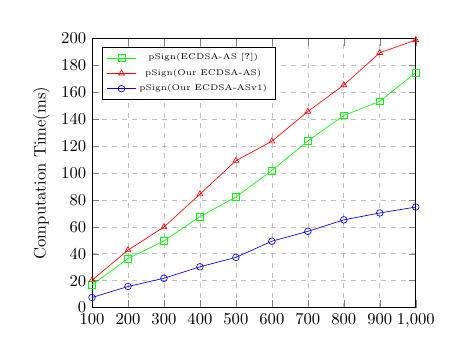
\begin{tikzpicture}[scale=0.6]
\begin{axis}[
    ylabel={Computation Time(ms)},
    xmin=100, xmax=1000,
    ymin=0, ymax=200,
    xtick={100,200,300,400,500,600,700,800,900,1000},
    ytick={0,20,40,60,80,100,120,140,160,180,200},
    legend pos=north west,
    ymajorgrids=true,
    grid style=dashed,
    xmajorgrids=true,
    grid style=dashed,
]
\addplot[
    color=green,
    mark=square,
    ]
    coordinates {(100,16.80)(200,36.44)(300,49.52)(400,67.61)(500,82.24)(600,101.88)(700,123.89)(800,142.80)(900,153.33)(1000,174.74)
    };

\addplot[
    color=red,
    mark=triangle,
    ]
    coordinates {(100,20.32)(200,42.70)(300,59.85)(400,84.29)(500,109.15)(600,123.66)(700,145.74)(800,165.46)(900,189.40)(1000,198.91)
    };

\addplot[
    color=blue,
    mark=o,
    ]
    coordinates {(100,7.46)(200,15.65)(300,21.77)(400,30.29)(500,37.30)(600,49.32)(700,56.66)(800,65.19)(900,70.33)(1000,74.74)
    };

    \legend{{\tiny pSign(ECDSA-AS~\cite{AumayrEEFHMMR20})},{\tiny pSign(Our ECDSA-AS)},{\tiny pSign(Our ECDSA-ASv1)}}
\end{axis}
\end{tikzpicture}
\end{minipage}
\hspace{0.15\textwidth}
\begin{minipage}[c]{0.3\textwidth}
\centering
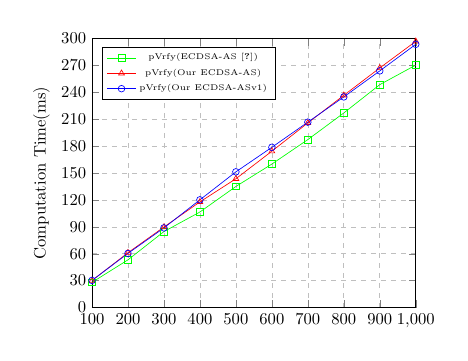
\begin{tikzpicture}[scale=0.6]
\begin{axis}[
    ylabel={Computation Time(ms)},
    xmin=100, xmax=1000,
    ymin=0, ymax=300,
    xtick={100,200,300,400,500,600,700,800,900,1000},
    ytick={0,30,60,90,120,150,180,210,240,270,300},
    legend pos=north west,
    ymajorgrids=true,
    grid style=dashed,
    xmajorgrids=true,
    grid style=dashed,
]
\addplot[
    color=green,
    mark=square,
    ]
    coordinates {(100,28.08)(200,53.20)(300,84.72)(400,106.56)(500,135.03)(600,160.03)(700,187.33)(800,217.03)(900,248.60)(1000, 270.41)
    };

\addplot[
    color=red,
    mark=triangle,
    ]
    coordinates {(100, 30.13)(200,61.13)(300,89.81)(400,117.81)(500,143.63)(600,174.35)(700,205.93)(800,236.70)(900,267.23)(1000,296.91)
    };

\addplot[
    color=blue,
    mark=o,
    ]
    coordinates {(100,30.23)(200,60.39)(300,88.82)(400,120.13)(500,151.34)(600,178.72)(700,206.79)(800,234.91)(900,263.94)(1000,293.57)
    };

    \legend{{\tiny pVrfy(ECDSA-AS~\cite{AumayrEEFHMMR20})},{\tiny pVrfy(Our ECDSA-AS)},{\tiny pVrfy(Our ECDSA-ASv1)}}
\end{axis}
\end{tikzpicture}
\end{minipage}
\centering
\caption{Efficiency comparison of pre-signing and pre-verification operation}
\label{fig3}
\end{figure}

\subsection{Experimental Analysis}

In order to evaluate the practical performance of our schemes, we implement the ECDSA-AS~\cite{AumayrEEFHMMR20}, and our ECDSA-AS and ECDSA-ASv1 based on the OpenSSL library. The program is executed on an Intel Core i5 CPU 2.3 GHz and 8GB RAM running macOS High Sierra 10.13.3 system.
 
As depicted in Figure~\ref{fig3}, we run our implementations on the standard NIST curves. We run ECDSA-AS~\cite{AumayrEEFHMMR20}, our ECDSA-AS and ECDSA-ASv1 many times respectively, and show the efficiency of online pre-signing and a verification operation. Based on the experimental data and analysis results, the average running times of all algorithms in ECDSA-AS and ECDSA-ASv1 are the level of microseconds. Especially, the average running times over 1000 executions of the online pre-signing operation in ECDSA-AS~\cite{AumayrEEFHMMR20}, our ECDSA-AS and ECDSA-ASv1 are 174.75 $\mu s$, 198.91 $\mu s$ and 74.74 $\mu s$. Therefore, our protocol can compare with the state-of-the-art ECDSA-AS~\cite{AumayrEEFHMMR20}.  

\section{Conclusions}

In this paper, we propose an ECDSA-AS and give the security proof based on ECDSA in the random oracle model. Compared with existing ECDSA-AS~\cite{Moreno-Sanchez2018,AumayrEEFHMMR20}, we can use the offline-proof technique to improve the efficiency of the online pre-signing algorithm and then construct two efficient ECDSA-AS called ECDSA-ASv1 and ECDSA-ASv2. For embedding the same hard relation $(I_Y,y)\in \mathsf{R}$, one proof $\pi_Z$ of hard relation $\mathsf{R}_Z$ used in the pre-signing phase can be used to pre-signing many messages. What's more, the pre-signing algorithms of ECDSA-ASv1/2 are similar to the original ECDSA signing algorithm except for modifying some parameters, they can completely reuse the hardware and software implementation of ECDSA and upgrade existing ECDSA applications friendly. In addition, ECDSA-ASv2 uses the same witness $y$ of hard relations $(I_Y,y)$ and $((G, Y, Q, Z), y)$, which is independent of the pre-signing key and random number used in pre-signing phase and need not be shared in constructing two-party AS so it can be transformed into two-party extension easily. Last, we define the two-party AS with interactive key generation, and following the fast two-party ECDSA~\cite{Lin17}, we construct an efficient two-party ECDSA-AS from our ECDSA-ASv2.  

\bibliography{mybib.bib}

\bibliographystyle{splncs03}

\newpage

\begin{center}
\huge{\textbf{Supplementary Material}}
\end{center}

\appendix
\renewcommand{\appendixname}{Appendix~\Alph{section}}

\section{Signature Scheme}

A signature scheme consists of three algorithms $\sum = (\mathsf{Gen},\mathsf{Sign},\mathsf{Vrfy})$ defined as follows. 

\begin{itemize}
\item $\mathsf{Gen}(1^\lambda)\rightarrow (vk,sk)$. The key generation algorithm takes the security parameter as input and outputs a verification key $vk$ and a secret key $sk$.
\item $\mathsf{Sign}_{sk}(m)\rightarrow \sigma$. The signing algorithm takes the secret key $sk$ and the message $m\in\{0,1\}^*$ as input, and outputs a signature $\sigma$. 
\item $\mathsf{Vrfy}_{vk}(m,\sigma)\rightarrow 0/1$. The verification algorithm takes the verification key $vk$, the message $m\in\{0,1\}^*$, and the signature $\sigma$ as input, and outputs either $0$ or $1$.
\end{itemize}

The correctness is that for any $(vk$, $sk)$ $\leftarrow$ $\mathsf{Gen}(1^\lambda)$ and $m\in\{0,1\}^*$, we have $\mathsf{Vrfy}_{vk}(m$, $\mathsf{Sign}_{sk}(m))\rightarrow 1$.

\begin{Definition}\emph{(SUF-CMA security).} A signature scheme $\sum$ is SUF–CMA secure if for every PPT adversary $\mathcal{A}$ there exists a negligible function $\mathsf{negl}$ such that: $\Pr[\text{sSigForge}_{\mathcal{A},\sum}(\lambda) = 1] \leq \mathsf{negl}(\lambda)$, where the experiment $\text{sSigForge}_{\mathcal{A},\sum}$ is defined as follows:
\end{Definition}

\begin{center}
\fbox{
\begin{tabular}{lll}
$\text{sSigForge}_{\mathcal{A},\sum}(\lambda)$ & \ \  & $\mathcal{O}_{\text{Sign}_{sk}}(m)$ \\
\cline{1-1} \cline{3-3}

$(vk,sk)\leftarrow \mathsf{Gen}(1^\lambda)$ & \ \  & $\sigma\leftarrow \mathsf{Sign}_{sk}(m)$ \\

$(m^*,\sigma^*)\leftarrow \mathcal{A}^{\mathcal{O}_{\text{Sign}_{sk}}(\cdot)}(vk)$ & \ \  & $\mathcal{Q}=\mathcal{Q}\cup \{m,\sigma\}$ \\

$\text{return} ((m^*,\sigma^*)\notin \mathcal{Q}\wedge \mathsf{Vrfy}_{vk}(m^*,\sigma^*))$ & \ \  & return $\sigma$ \\

\end{tabular}}
\end{center}

\section{Two-party Signature}

We review two-party signature and its security in~\cite{Lin17,CCLST19}. The two-party signature $\Pi=(\mathsf{IGen},\mathsf{ISign},\mathsf{Vrfy})$ consists of two distributed protocols and a verification algorithm as follows:

\begin{itemize}
\item $\mathsf{IGen}(pp)\rightarrow ((sk_0,vk);(sk_1,vk))$. The interactive key generation protocol takes in the public parameter $pp$ and outputs the pre-signing key and verification key $(sk_0,vk);(sk_1,vk)$ for each party $P_i,i=0,1$.

\item $\mathsf{ISign}_{\langle sk_0, sk_1\rangle}(m) \rightarrow \sigma$. The interactive signing protocol takes in common message $m\in\{0,1\}^*$ and pre-signing key $sk_0,sk_1$ from each party $P_i,i=0,1$ and output the signature $\sigma$.

\item $\mathsf{Vrfy}_{vk}(m,\sigma)\rightarrow 0/1$. The verification algorithm takes the verification key $vk$, the message $m\in\{0,1\}^*$, and the signature $\sigma$ as input, and outputs either $0$ or $1$.
\end{itemize}

We review the security definition of two-party signature in~\cite{Lin17,CCLST19}. In the experiment $\text{SigForge}^b_{\mathcal{A},\Pi}(\lambda)$,\ $b\in\{0,1\}$ , a PPT adversary $\mathcal{A}$ corrupting the party $P_b$ in protocol $\Pi$ can interact with an oracle $\mathcal{O}_{\Pi^b}(\cdot,\cdot)$ to generate the verification key and pre-signing keys and sign any messages concurrently, which executes as another party $P_{1-b}$. $\mathcal{O}_{\Pi^b}(\cdot,\cdot)$ is defined such that the interactive key generation protocol $\Pi^b_{\text{IKG}}$ is first run once and then the signing protocol $\Pi^b_{\text{ISign}_{\langle sk_{1-b},\cdot\rangle}}$ can be executed concurrently. 

In the key generation phase, the interactive key generation oracle $\Pi^b_{\text{IKG}}(\cdot,\cdot)$ works as follows: 
\begin{itemize}
\item Upon receiving $(0,0)$ first, the oracle initializes a machine $M$ and acts as the party $P_{1-b}$ to reply. 
\item Upon receiving $(0,m)$, the oracle hands $M$ the message $m$ as its next incoming message and returns $M$'s reply. 
\item Upon receiving $(sid,m)$ is received where $sid \not= 0$, the oracle returns $\bot$.
\end{itemize}

In the signing phase, the interactive signing oracle $\Pi^b_{\text{ISign}_{\langle sk_{1-b},\cdot\rangle}}(\cdot,\cdot)$ works as follows:
\begin{itemize}
\item Upon receiving $(sid,m)$ and this is the first oracle query with this identifier $sid$, the oracle initializes a new machine $M_{sid}$ with the key share and any state stored by $M$ at the end of the key generation phase. The $M_{sid}$ executes as the party $P_{1-b}$ with session identifier $sid$ and input message $m$ to be signed.  
\item Upon receiving  $(sid,m)$ and this is not the first oracle query with this identifier $sid$, the oracle hands $M_{sid}$ the incoming message $m$ and returns the next message sent by $M_{sid}$. If $M_{sid}$ concludes, then the output obtained by $M_{sid}$ is returned.
\end{itemize}

The adversary $\mathcal{A}$ controlling $P_b$ with oracle access to $\mathcal{O}_{\Pi^b}(\cdot,\cdot)$ ``wins'' if it can forge a signature on a message that is not queried. For a detailed explanation we refer the reader to~\cite{Lin17}. 

\begin{Definition}~\label{two-party signature EUF-CMA}
The two-party signature $\Pi=(\mathsf{IGen},\mathsf{ISign},\mathsf{Vrfy})$ is secure if for every PPT adversary $\mathcal{A}$ there exists a negligible function $\mathsf{negl}$ for $b\in\{0,1\}$, such that: $\Pr[\text{SigForge}^b_{\mathcal{A},\Pi}(\lambda) = 1] \leq \mathsf{negl}(\lambda)$, where the experiment $\text{SigForge}^b_{\mathcal{A},\Pi}$ is defined as follows:
\end{Definition}

\begin{center}
\fbox{
\begin{tabular}{lll}
$\text{SigForge}^b_{\mathcal{A},\Pi}(\lambda)$& \ \  & $\Pi^b_{\text{IKG}}(\cdot,\cdot)$ \\
\cline{1-1} \cline{3-3} 
$(vk,sk_b)\leftarrow \mathcal{A}^{\Pi^b_{\text{IKG}}(\cdot,\cdot)}(1^\lambda)$ & \ \  & $((vk,sk_{b});((vk,sk_{1-b}))\leftarrow \Pi^b_{\text{IKG}}(\cdot,\cdot)$ \\

$(m^*,\sigma^*)\leftarrow \mathcal{A}^{\Pi^b_{\text{ISign}_{\langle sk_{1-b},\cdot\rangle}}(\cdot,\cdot)}(vk,sk_b)$ & \ \  &  \\

return $\mathsf{Vrfy}_{vk}(m^*,\sigma^*) = 1 \wedge m^* \notin \mathcal{Q}$ & \ \  & $\Pi^b_{\text{ISign}_{\langle sk_{1-b},\cdot\rangle}}(sid,m)$ \\
\cline{3-3} 
 & \ \  & $\sigma\leftarrow \Pi^b_{\text{ISign}_{\langle sk_{1-b},\cdot\rangle}}(sid,m)$ \\

 & \ \  & $\mathcal{Q}=\mathcal{Q}\cup \{m\}$ \\
\end{tabular}}
\end{center}

\section{Hard Relation and Zero-Knowledge Proof}~\label{Hard Relation and Zero-Knowledge Proof}

We recall the definition of a hard relation $\mathsf{R}$ with statement/witness pairs $(stat=(G$, $Y),y)$, where $Y=yG$~\cite{AumayrEEFHMMR20}. Let $\mathsf{L}_\mathsf{R}$ be the associated language defined as $\mathsf{L}_\mathsf{R}= \{(G,Y)| \exists\  y$ s.t. $((G,Y),y) \in \mathsf{R}\}$. We say that $\mathsf{R}$ is a hard relation if the following holds: (i) There exists a PPT sampling algorithm $\mathsf{GenR}(1^\lambda)$ that on input $1^\lambda$ outputs a statement/witness pair $((G,Y),y) \in \mathsf{R}$; (ii) The relation is poly-time decidable; (iii) For all PPT $\mathcal{A}$ the probability of $\mathcal{A}$ on input $(G,Y)$ outputting $y$ is negligible.

We also recall the definition of a non-interactive zero-knowledge proof of knowledge with online extractors as introduced in~\cite{Fischlin05}. The online extractability property allows for extraction of a witness $y$ for an instance $(G,Y)$ from a proof $\pi$ in the random oracle model and is useful for models where the rewinding proof technique is not allowed, such as UC. We will need this property in order to prove our ECDSA-AS scheme is secure. More formally, a pair $(\mathsf{P}, \mathsf{V})$ of PPT algorithms is called a non-interactive zero-knowledge proof of knowledge with an online extractor for a relation $\mathsf{R}$, random oracle $\mathcal{H}$ and security parameter $\lambda$ if the following holds: (i) Completeness: For any $((G,Y),y) \in \mathsf{R}$, it holds that $\mathsf{V}((G,Y), \mathsf{P}((G,Y), y)) = 1$; (ii) Zero knowledge: There exists a PPT simulator $S$, which on input $(G,Y)$ can simulate the proof $\pi$ for any $((G,Y),y) \in \mathsf{R}$. (iii) Online Extractor: There exists a PPT online extractor $\mathsf{K}$ with access to the sequence of queries to the random oracle and its answers, such that given $((G,Y),\pi)$ , the algorithm $\mathsf{K}$ can extract the witness $y$ with $((G,Y),y) \in \mathsf{R}$. 

We review some hard relations and their corresponding zero-knowledge proof following~\cite{Lin17}.
\begin{itemize}
\item[1.]\emph{Proof that a Paillier public-key was generated correctly:} define the relation of valid Paillier public keys: 
$$\mathsf{R}_{\text{P}} = \{(N,\phi(N)) | \mathsf{gcd}(N,\phi(N)) = 1\}$$
\item[2.]\emph{Proof of knowledge of the discrete log of an Elliptic-curve point:} define the
relation of discrete log values (relative to the given group).
$$\mathsf{R}_{\text{DL}} =\{(\mathbb{G},G,q,P,w)|P =w\cdot G\} $$
\item[3.]\emph{Proof of knowledge of the equality of discrete logs of two Elliptic-curve points:} define the relation of two discrete log values (relative to the given group).
$$\mathsf{R}_{\text{EDL}} =\{(\mathbb{G},G,Q,q,X,Y,w)|X =w\cdot G\wedge Y=w\cdot Q\} $$
\item[4.]\emph{Prove in zero-knowledge that a value encrypted in a given Paillier and the ciphertext is the discrete log of a given Elliptic curve point:} define the language where $pk$ is a given Paillier public key and $sk$ is its associated private key.
$$\mathsf{L}_{\text{PDL}} = \{(c,pk,Q_1,\mathbb{G},G,q) | \exists\  (x_1,r)\ \text{s.t.}\ c=\mathsf{Enc}(pk,x;r)\wedge Q_1 =x_1\cdot G \wedge x_1 \in \mathbb{Z}_q\}$$

\end{itemize}

\section{Some Functionalities}~\label{Some Functionalities}

We review the ECDSA ideal functionality $\mathcal{F}_{\text{ECDSA}}$~\cite{Lin17} between two parties $P_0$ and $P_1$ as follows. The functionality is defined with two functions: key generation and signing. The key generation is called once, and then any arbitrary number of signing operations can be carried out with the generated key.

\begin{center}
\fbox{\parbox{0.9\textwidth}{
\textbf{The ECDSA Functionality $\mathcal{F}_{\text{ECDSA}}$.}
\begin{itemize}
\item Upon receiving $\mathsf{Gen}(\mathbb{G}, G, q)$ from two parties $P_0,P_1$, then:

\begin{itemize}
\item[1.]Generate a pair of ECDSA keys $(x, Q)$, where $x\leftarrow \mathbb{Z}^*_q$ is the secret signing key, and $Q = x\cdot G$ is the verification key.
\item[2.]Send $Q$ to both parties.
\item[3.]Ignore future calls to $\mathsf{Gen}$.
\end{itemize}

\item  Upon receiving $\mathsf{Sign}(sid,m)$ from $P_0,P_1$, if $\mathsf{Gen}$ was already
called and $sid$ has not been stored, then:

\begin{itemize}
\item[1.]Compute an ECDSA signature $(r, s)$ on $m$. 
\item[2.]Send $(r, s)$ to both parties, and store $(sid, m)$.
\end{itemize}

\end{itemize}}}
\end{center}

We review some ideal functionalities used in~\cite{Lin17,CCLST19}, including the ideal commitment functionality $\mathcal{F}_{\text{com}}$, the ideal zero-knowledge functionality $\mathcal{F}_{\text{zk}}$, and the committed non-interactive zero-knowledge functionality $\mathcal{F}^\mathsf{R}_{\text{com\text{-}zk}}$. For a detailed explanation of these ideal functionalities we refer the reader to~\cite{Lin17}.

The ideal commitment functionality $\mathcal{F}_{\text{com}}$~\cite{Lin11,Fuj16} works with parties $P_0$ and $P_1$, formally defined as follows.
\begin{center}
\fbox{\parbox{0.9\textwidth}{
\textbf{The Commitment Functionality $\mathcal{F}_{\text{com}}$.}
\begin{itemize}
\item Upon receiving $(\mathsf{commit},sid,x)$ from party $P_i$ (for $i \in \{0,1\}$), record $(sid,i,x)$ and send $(\mathsf{receipt},sid)$ to party $P_{1-i}$ . If $(\mathsf{commit},sid,*)$ is already stored, then ignore the message.
\item Upon receiving $(\mathsf{decommit},sid)$ from party $P_i$, if $(sid,i,x)$ is recorded then send $(\mathsf{decommit},sid,x)$ to party $P_{1-i}$.
\end{itemize}}}
\end{center}

A standard ideal zero-knowledge functionality~\cite{HL10} is defined by $((x,w)$, $\emptyset)$ $\leftarrow$ $(\emptyset,(x,\mathsf{R}(x,w)))$. For a relation $\mathsf{R}$, the ideal zero-knowledge functionality is denoted by $\mathcal{F}^\mathsf{R}_{\text{zk}}$, formally defined as follows. 
\begin{center}
\fbox{\parbox{0.9\textwidth}{
\textbf{The Zero Knowledge Functionality $\mathcal{F}^\mathsf{R}_{\text{zk}}$ for Relation $\mathsf{R}$.}
\begin{itemize}
\item Upon receiving $(\mathsf{prove},sid,x,w)$ from a party $P_i$ (for $i \in \{0,1\}$): if $(x,w)\notin \mathsf{R}$ or $sid$ has been previously used then ignore the message. Otherwise, send $(\mathsf{proof},sid,x)$ to party $P_{1-i}$.
\end{itemize}}}
\end{center}

For a relation $\mathsf{R}$, the commitments to non-interactive zero-knowledge proofs of knowledge used by the ideal commitment functionality $\mathcal{F}_{\text{com}}$ is denoted by $\mathcal{F}^\mathsf{R}_{\text{com\text{-}zk}}$, formally defined as follows.
\begin{center}
\fbox{\parbox{0.9\textwidth}{
\textbf{The Committed NIZK Functionality $\mathcal{F}^\mathsf{R}_{\text{com\text{-}zk}}$ for Relation $\mathsf{R}$.}
\begin{itemize}
\item Upon receiving $(\mathsf{com\text{-}prove},sid,x,w)$ from a party $P_i$ (for $i \in \{0,1\}$): if $(x,w) \notin \mathsf{R}$ or $sid$ has been previously used then ignore the message. Otherwise, store $(sid,i,x)$ and send $(\mathsf{proof\text{-}receipt},sid)$ to $P_{1-i}$.
\item Upon receiving $(\mathsf{decom\text{-}proof},sid)$ from a party $P_i$ (for $i\in \{0,1\}$): if $(sid,i,x)$ has been stored then send $(\mathsf{decom\text{-}proof},sid,x)$ to $P_{1-i}$ 
\end{itemize}}}
\end{center}

% \section{Applications}

% \subsection{Atomic Swaps}

% An atomic swap can be defined between two users $u_1$ and $u_2$ who want to exchange two different cryptocurrencies $c_1$ and $c_2$. The crucial point of the exchange is ensuring fairness, i.e., either both parties receive their expected output or none do. In [23], an atomic swap protocol is presented with the following steps.

% \subsection{Payment Channel Networks}




\end{document}

